\documentclass[11pt]{article}
\usepackage[utf8]{inputenc}
\usepackage[margin=1in]{geometry}
\usepackage{amsmath,amssymb}
\usepackage{graphicx}
\usepackage{booktabs}
\usepackage{multirow}
\usepackage{tikz}
\usepackage{caption}
\usepackage{url}
\usepackage[hidelinks]{hyperref}

\usetikzlibrary{arrows.meta,positioning,fit,backgrounds,calc,decorations.pathreplacing}
\graphicspath{{../results/figures/}}

\captionsetup{font=small}

\title{Decision Transformer for Sequential Portfolio Allocation:\\
An Offline Reinforcement Learning Study on 30 Years of Market Data}
\author{Md.\ Shahriar Islam Bhuiyan\\
Section: \texttt{<section>} \qquad Student ID: \texttt{<id>}\\
\texttt{shojeb.bhuiyan@gmail.com}}
\date{}

\begin{document}

\maketitle

\begin{abstract}
Allocating capital across many assets is a sequential decision problem, but the obvious way
to solve it with reinforcement learning---letting an agent explore a live market---is
impossible: every exploratory trade costs real money and no historical regime can be replayed.
Offline reinforcement learning and, more recently, return-conditioned sequence modelling
promise a way out, and the Decision Transformer (DT) in particular claims that simply
conditioning an autoregressive model on a desired Return-to-Go (RTG) is enough to recover
good behaviour from a fixed dataset. In this project we test that claim on a long-only,
cost-aware, multi-asset allocation task built from a 30-year daily-close dataset. We
construct a 14-asset investable universe with 6{,}369 trading days, engineer a 2{,}580-dimensional
state from 129 daily features over a 20-day lookback, synthesise 3{,}600 offline trajectories
from a mixture of 18 behaviour policies, and train eight learned allocators---Decision
Transformer, transformer behaviour cloning, TD3+BC, IQL, CQL, PPO, SAC and A2C---across five
random seeds each, for a total of 40 checkpoints per universe, then backtest all of them
against six classical baselines on a strictly held-out 2020--2025 window with a 10\,bp
proportional transaction cost. The results are consistently negative for the learned
allocators and informative about why: no learned method beats the cost-aware equal-weight
portfolio (Sharpe $1.118$); DT reaches Sharpe $0.966\pm0.133$ and is statistically
indistinguishable from its own RTG-free control ($0.976\pm0.106$); sweeping the target RTG
across training-return quantiles moves realised Sharpe by less than $0.04$ and in the wrong
direction, showing that the return-conditioning channel is essentially unused; a weight-level
analysis explains the shortfall---on four of five seeds DT's average book is equal weight plus
noise (Herfindahl $0.0715$ against a uniform $0.0714$), so the model rediscovers the baseline's
allocation and then pays turnover to keep re-deriving it; a
transaction-cost ablation shows DT still trails equal weight by $0.07$ Sharpe even at zero
cost, so turnover explains only about half of the gap; and a context-length ablation over
$K \in \{10,20,30,50\}$ moves the imitation loss by $0.3\%$ while closing none of the gap.
Repeating the entire
pipeline on a second universe that adds Bitcoin and aluminium reproduces every qualitative
conclusion.
\end{abstract}

\section{Introduction}

Portfolio allocation asks how to split one unit of capital across $N$ assets on every trading
day so that long-run wealth grows quickly without exposing the investor to ruinous drawdowns.
It is naturally sequential: today's weights determine tomorrow's starting holdings, and every
change of mind is taxed by transaction costs, so a decision cannot be evaluated in isolation.
This makes the problem a textbook fit for reinforcement learning (RL), and a poor fit for the
standard RL \emph{protocol}. An online agent learns by acting, and acting in a market means
losing real money on every exploratory trade; worse, markets are non-stationary and
non-repeatable, so the environment an agent explored last year no longer exists. The
practical consequence is that essentially all realistic financial RL is \emph{offline}: the
agent must learn from a fixed record of what some other strategy did. Getting this right
matters well beyond finance---pension funds, index providers and robo-advisors already
allocate trillions using rules that a learned allocator would have to beat---and it is also a
demanding stress test for offline RL itself, because the environment is exogenous (the agent
cannot move prices), the reward is nearly a martingale, and a trivial policy (hold
$1/N$ forever) is a famously strong baseline \cite{demiguel2009optimal}.

A long line of work has attacked this problem. Moody and Saffell \cite{moody2001learning}
introduced direct (policy-gradient) reinforcement for trading and showed that optimising a
differentiable Sharpe-like utility beats training a return forecaster and trading its output;
their setting, however, is single-asset and predates deep function approximation. Deng et
al.\ \cite{deng2016deep} added deep representation learning on top of direct RL and improved
signal extraction, but still on individual futures contracts and without an explicit budget
constraint. Jiang et al.\ \cite{jiang2017deep} are the closest classical antecedent of our
setup: they define the portfolio-vector-memory MDP with simplex actions and a
transaction-cost-adjusted log return, which we adopt almost unchanged, but they evaluate on a
short cryptocurrency window in which nearly every strategy was profitable, so the baseline
bar was low. Zhang et al.\ \cite{zhang2020deep} ran DQN, PG and A2C over 50 liquid futures
with careful cost modelling and reported genuine but small risk-adjusted gains---their study is
methodologically the most careful of the group, and notably also finds that performance
degrades quickly as costs rise. Yang et al.\ \cite{yang2020deep} ensembled PPO, A2C and DDPG
for 30 Dow stocks and report a Sharpe above the index, but their agents interact with a
simulator built from the same prices they are evaluated on, which is exactly the online
protocol that is unavailable in practice; the accompanying FinRL library
\cite{liu2021finrl} has made this protocol the de facto standard and, in our view,
has propagated its optimism. On the algorithmic side, offline RL has developed principled
answers to the distribution-shift problem that dooms naive off-policy learning on static data
\cite{levine2020offline}: CQL \cite{kumar2020conservative} penalises over-estimated
$Q$-values on out-of-distribution actions, IQL \cite{kostrikov2022offline} avoids querying
unseen actions altogether by fitting an expectile value function, and TD3+BC
\cite{fujimoto2021minimalist} shows that a single behaviour-cloning term added to TD3
\cite{fujimoto2018addressing} is a surprisingly strong baseline. Orthogonally, the Decision
Transformer \cite{chen2021decision} and Trajectory Transformer
\cite{janner2021trajectory} discard value learning entirely and recast offline RL as
autoregressive sequence modelling over $(\hat{R}_t, s_t, a_t)$ tokens with a GPT-style causal
transformer \cite{vaswani2017attention}; conditioning on a high target return at inference is
supposed to elicit high-return behaviour. Their published evidence is drawn from Atari,
D4RL locomotion and Key-to-Door---dense, stationary, endogenous environments that differ from
markets in every property that matters here. Closest to our architecture, Kisiel and Gorse
\cite{kisiel2022portfolio} apply an encoder--decoder transformer directly to asset allocation
and train it end to end on a transaction-cost-penalised Sharpe objective, outperforming LSTM
alternatives; theirs, however, is a supervised allocator rather than a return-conditioned
sequence model, so it tells us nothing about whether the Return-to-Go channel carries
information. Studies that do apply Decision Transformers to allocation typically report
favourable numbers against a single index benchmark, on one asset universe, with one seed, and
without an RTG-free control, so it is impossible to tell whether the transformer or the return
conditioning did any work.

That gap is what this project addresses. Every ingredient needed to answer the question
honestly---an RTG-free control that is architecturally identical to DT, several seeds, a
transaction cost, a genuinely held-out multi-year window, classical baselines that are
actually competitive, and significance testing that accounts for the number of strategies
tried---is individually standard, yet we are not aware of a portfolio study that combines them.
Without the RTG-free control, DT's score cannot be separated from plain imitation of the
behaviour data; without several seeds, a difference of $0.1$ Sharpe is noise; without a
transaction cost, any high-turnover policy looks good; and without a strong $1/N$ baseline,
a mediocre allocator looks like a success. We therefore rebuilt the pipeline end to end so
that each of these controls is present simultaneously, and we report what it shows even
though the headline finding is negative. A negative result obtained under proper controls is
more useful to the next practitioner than a positive one obtained without them, and the
ablations tell us specifically \emph{which} link in the DT story breaks on this task.

\subsection{Our Contribution}
\begin{enumerate}
  \item We formalise long-only, cost-aware, daily multi-asset allocation as a finite-horizon
        MDP with simplex actions and a net-log-growth reward, and implement it as a
        dependency-free NumPy environment in which every strategy---classical, cloned or
        learned---is the same callable $(t, s_t) \mapsto a_t \in \Delta^{N-1}$, so all
        comparisons run through identical backtest code.
  \item We build a reproducible offline dataset from a public 30-year daily-close dataset
        \cite{islam2025dataset}: NYSE-calendar alignment, a synthetic 10-year Treasury
        total-return series derived from yields, a floored T-bill cash asset, 129 engineered
        daily features flattened over a 20-day lookback into $s_t \in \mathbb{R}^{2580}$, and
        3{,}600 episodes of 252 days rolled out from a mixture of 18 behaviour policies.
  \item We train and evaluate \textbf{eight} learned allocators (Decision Transformer,
        transformer BC, TD3+BC, IQL, CQL, PPO, SAC, A2C) at \textbf{five seeds} each and
        compare them with \textbf{six} classical baselines under an identical protocol, giving
        40 learned checkpoints and 46 evaluated strategies per universe.
  \item We report a full ablation suite: RTG conditioning on/off (DT vs.\ an architecturally
        identical control), target-RTG quantile, Decision Transformer context length
        $K \in \{10,20,30,50\}$, transaction cost $\mu \in \{0, 5, 10, 25\}$\,bp, and an
        entire second asset universe that adds Bitcoin and aluminium.
  \item We quantify significance properly---circular block-bootstrap confidence intervals on
        Sharpe differences, the Ledoit--Wolf robust Sharpe test \cite{ledoit2008robust}, and
        the deflated Sharpe ratio \cite{bailey2014deflated}---and document the RL correctness
        bugs (self-referential Bellman targets, frozen target networks, a batch-wise instead
        of action-wise CQL penalty) that had to be fixed before any of the baseline numbers
        were meaningful.
\end{enumerate}

\section{Material and Methods}

Figure~\ref{fig:block} is the graphical abstract of the project. The pipeline runs strictly
left to right and every stage hands off through files on disk rather than in-memory objects,
so any stage can be re-run on its own once the previous stage's artefacts exist.
\textbf{(1) Data preparation} reads the three raw CSVs, reindexes the union calendar onto NYSE
trading days (defined as days on which the S\&P~500 close is present), forward-fills gaps for
at most five sessions, synthesises a 10-year Treasury total-return index from the yield
series and a cash index from the 13-week T-bill yield, and splits the columns into a
14-asset \emph{investable} universe and a larger \emph{feature-only} set.
\textbf{(2) Feature engineering} turns those prices into 129 daily features---returns, MACD,
RSI, Bollinger \%b, realised volatility at two horizons, cross-sectional momentum ranks,
macro indicators and crisis-event flags---then flattens a 20-day sliding window into a single
state vector $s_t \in \mathbb{R}^{2580}$ and standardises it with training-split statistics
only. \textbf{(3) Trajectory synthesis} rolls 18 behaviour policies through the portfolio
environment over 200 sampled 252-day windows each, producing 3{,}600 episodes of
$(\hat{R}_t, s_t, a_t, r_t)$ tuples. \textbf{(4) Offline training} fits the Decision
Transformer and seven baselines to that buffer, five seeds apiece, writing one checkpoint per
(model, seed) pair plus a manifest. \textbf{(5) Evaluation} loads every successful checkpoint,
wraps it as a policy callable, and replays it through the same environment on the held-out
window, producing metric tables, significance tests, walk-forward folds and the ablation
sweeps. The dashed feedback arrow marks the only loop in the diagram: the ablation stage
re-enters training when it needs a model retrained at a different context length.

\begin{figure}[t]
\centering
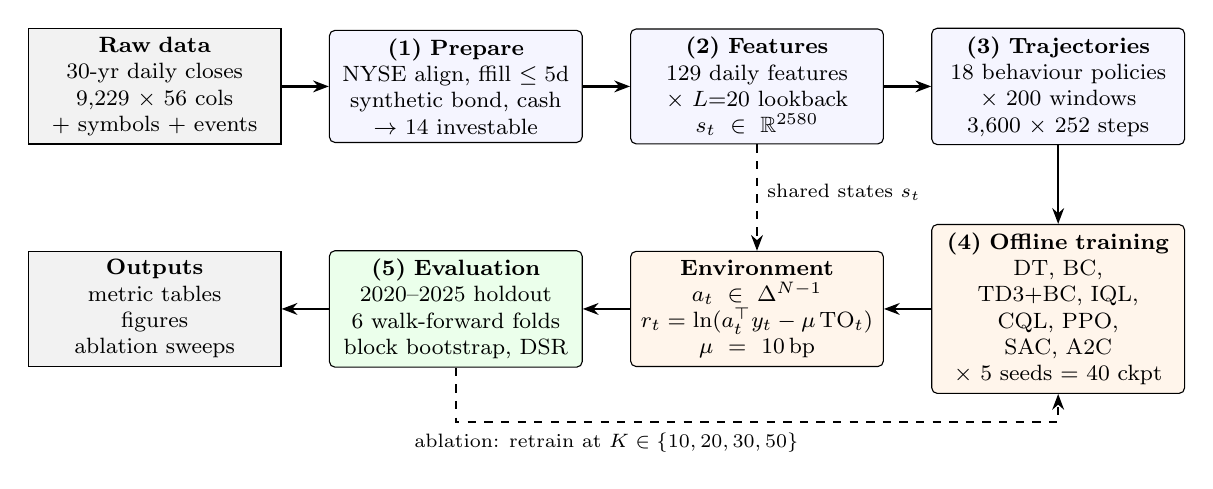
\begin{tikzpicture}[
  font=\footnotesize,
  box/.style={draw, rounded corners=2pt, align=center, minimum height=9mm,
              inner sep=3pt, text width=30mm, fill=blue!4},
  data/.style={draw, align=center, minimum height=7mm, inner sep=3pt,
               text width=30mm, fill=gray!10},
  arr/.style={-{Stealth[length=2mm]}, thick},
  node distance=5mm and 6mm
]
\node[data] (raw) {\textbf{Raw data}\\ 30-yr daily closes\\ 9{,}229 $\times$ 56 cols\\ + symbols + events};
\node[box, right=of raw] (prep) {\textbf{(1) Prepare}\\ NYSE align, ffill $\le 5$d\\ synthetic bond, cash\\ $\rightarrow$ 14 investable};
\node[box, right=of prep] (feat) {\textbf{(2) Features}\\ 129 daily features\\ $\times$ $L{=}20$ lookback\\ $s_t \in \mathbb{R}^{2580}$};
\node[box, right=of feat] (traj) {\textbf{(3) Trajectories}\\ 18 behaviour policies\\ $\times$ 200 windows\\ 3{,}600 $\times$ 252 steps};

\node[box, below=10mm of traj, fill=orange!8] (train)
  {\textbf{(4) Offline training}\\ DT, BC, TD3+BC, IQL,\\ CQL, PPO, SAC, A2C\\ $\times$ 5 seeds = 40 ckpt};
\node[box, left=of train, fill=orange!8] (env)
  {\textbf{Environment}\\ $a_t \in \Delta^{N-1}$\\ $r_t = \ln(a_t^\top y_t - \mu\,\mathrm{TO}_t)$\\ $\mu = 10$\,bp};
\node[box, left=of env, fill=green!8] (eval)
  {\textbf{(5) Evaluation}\\ 2020--2025 holdout\\ 6 walk-forward folds\\ block bootstrap, DSR};
\node[data, left=of eval] (out)
  {\textbf{Outputs}\\ metric tables\\ figures\\ ablation sweeps};

\draw[arr] (raw) -- (prep);
\draw[arr] (prep) -- (feat);
\draw[arr] (feat) -- (traj);
\draw[arr] (traj) -- (train);
\draw[arr] (train) -- (env);
\draw[arr] (env) -- (eval);
\draw[arr] (eval) -- (out);
% state matrix is consumed by the environment as well as by the trajectory stage
\draw[arr, dashed] (feat.south) -- node[right, pos=0.45, font=\scriptsize]
  {shared states $s_t$} (env.north);
% context-length ablation re-enters training
\draw[arr, dashed] (eval.south) |- ($(env.south)+(0,-7mm)$)
  node[below, pos=0.75, font=\scriptsize] {ablation: retrain at $K \in \{10,20,30,50\}$}
  -| (train.south);
\end{tikzpicture}
\caption{Graphical abstract of the pipeline. Stages (1)--(3) turn a raw 30-year
daily-close dataset into a 3{,}600-episode offline buffer of $(\hat{R},s,a,r)$ tuples;
stage (4) fits eight learned allocators at five seeds each; stage (5) replays every
checkpoint through the \emph{same} cost-aware portfolio environment used to generate the
data, on a window the learners never saw. Every arrow is a file on disk, so each stage is
independently reproducible. The dashed loop is the context-length ablation, which is the only
part of the study that requires retraining.}
\label{fig:block}
\end{figure}

\subsection{Dataset Description}
\label{sec:data}

All market data comes from the public Kaggle dataset \emph{30 Years of Stock Market Data}
by Asim Islam \cite{islam2025dataset}, available at
\url{https://www.kaggle.com/datasets/asimislam/30-yrs-stock-market-data}. It contains three
files, summarised in Table~\ref{tab:dataset}: a wide matrix of daily closing prices for 56
instruments, a symbol metadata table giving each column's ticker, asset class and unit, and a
table of 11 dated financial crises which we convert into event-window indicator features. We
chose this dataset for three reasons. First, its span (31 calendar years) is long enough to
contain several distinct market regimes---the dot-com collapse, the 2008 credit crisis, the
COVID-19 crash, and the 2022 rate-hike drawdown---so a chronological train/test split is a
real distribution shift rather than a formality. Second, it is genuinely multi-asset: equities,
mutual funds, ETFs, precious and industrial metals, energy, currencies, crypto and the full
Treasury yield curve appear in one aligned frame, which is what makes a \emph{diversified}
allocation problem possible at all. Third, it is a single self-contained download, so the
entire study can be reproduced without a paid data vendor.

\begin{table}[t]
\centering
\caption{Properties of the raw dataset \cite{islam2025dataset} and of the derived
Universe~A used for all headline results. ``Feature-only'' columns are observable to the
agent through the state vector but are not investable---either because they are indices or
yields with no tradable total return in the file, or because they contain invalid prices
(WTI crude printed $-37.63$ on 2020-04-20).}
\label{tab:dataset}
\small
\begin{tabular}{lll}
\toprule
& \textbf{Property} & \textbf{Value} \\
\midrule
\multirow{6}{*}{\rotatebox{90}{\textbf{Raw}}}
 & Source & Kaggle, \texttt{asimislam/30-yrs-stock-market-data} \\
 & Files & prices, symbol metadata, financial events \\
 & Rows $\times$ columns & $9{,}229 \times 56$ (daily closes) \\
 & Calendar span & 1995-01-02 -- 2025-12-30 \\
 & Asset classes & indices, stocks, ETFs/funds, metals, energy, FX, crypto, Treasuries \\
 & Financial events & 11 dated crises (1997 Asia $\rightarrow$ 2025 tariffs) \\
\midrule
\multirow{7}{*}{\rotatebox{90}{\textbf{Universe A}}}
 & Investable assets $N$ & 14 \\
 & Trading days & 6{,}369 (2000-09-01 -- 2025-12-30, NYSE calendar) \\
 & State dates after lookback & 6{,}330 \\
 & Daily features & 129 \\
 & Lookback $L$ & 20 days $\Rightarrow$ $d_s = 129 \times 20 = 2{,}580$ \\
 & Feature-only series & VIX, USD, WTI, Brent, natural gas, DAX/FTSE/HSI/Nasdaq/NYSE, yields \\
 & Missing-data rule & forward-fill $\le 5$ sessions, then drop the leading window \\
\midrule
\multirow{3}{*}{\rotatebox{90}{\textbf{Split}}}
 & Train & 2000-09-01 -- 2016-12-31 \\
 & Validation & 2017-01-01 -- 2019-12-31 \\
 & Test (held out) & 2020-01-01 -- 2025-12-30 (1{,}507 trading days) \\
\bottomrule
\end{tabular}
\end{table}

\paragraph{Universe construction.}
Not every column in the file can be held in a portfolio. Indices such as the DAX or the VIX
have no investable total return in this dataset, Treasury columns are \emph{yields} rather than
prices, and WTI crude contains a negative close on 2020-04-20 that makes a gross return
undefined. We therefore split the columns in two. The \textbf{investable universe}
(``Universe~A'', $N=14$) consists of nine equity-like instruments (S\&P~500 ETF, Fidelity Blue
Chip Growth Fund, Apple, Microsoft, Amazon, Nvidia, JP Morgan Chase, Walmart, Fidelity Select
Energy Portfolio), three metals (gold, silver, copper), one synthetic 10-year Treasury
total-return index built from the yield series via the duration approximation
$r^{\text{bond}}_t \approx -D\,\Delta y^{10\text{Y}}_t + y^{10\text{Y}}_{t-1}/252$ with $D=8$,
and one cash asset accruing $\max(y^{\text{bill}}_t/100/252,\,0)$ per day (the floor is needed
because the 13-week bill yield printed $-0.105\%$ on 2020-03-26). Universe~A starts on
2000-09-01, the first date on which all three metals are available. Everything else in the
file---VIX, the US dollar index, WTI and Brent, natural gas, the four foreign equity indices,
and the rest of the yield curve---enters the \textbf{feature-only} set: the agent observes it
but cannot allocate to it. A second universe (``Universe~B'') adds Bitcoin and aluminium and
therefore starts on 2014-09-17, the first date on which Bitcoin is quoted; it is used in
Section~\ref{sec:universeb} as a robustness check and is otherwise held out of the headline
numbers.

\paragraph{Feature description.}
The 129 daily features decompose as follows. \emph{(i) Returns} ($14$ features): the one-day
simple return of each investable asset. \emph{(ii) Technical indicators} ($14 \times 5 = 70$):
for each asset, the MACD histogram normalised by price ($12/26/9$ EMA spans), RSI(14),
Bollinger \%b over a 20-day window, and annualised realised volatility at 20 and 60 days.
These are all close-based, which is a constraint of the dataset---it carries no volume, so
volume- or microstructure-based indicators are impossible. \emph{(iii) Cross-sectional
momentum ranks} ($14 \times 2 = 28$): the percentile rank of each asset's trailing cumulative
return within the universe at 60- and 120-day horizons, which gives the model a relative
rather than absolute momentum signal. \emph{(iv) Macro features} ($6$): the VIX level, the
daily US dollar return, the 10Y--3M and 30Y--5Y term spreads, and WTI and natural-gas returns.
\emph{(v) Event flags} ($11$): one binary indicator per crisis in the events file, switched on
for a $\pm 30$-day window around the event date, which lets the model recognise regime
boundaries it would otherwise have to infer. A state is the concatenation of these 129
features over the trailing 20 sessions, so $s_t$ contains both the current cross-section and
its recent trajectory; all features are computed from information available at or before day
$t$, and a dedicated unit test asserts that shifting any feature forward in time changes the
result (a no-lookahead check).

\begin{figure}[t]
\centering
\begin{minipage}[t]{0.48\textwidth}
\centering
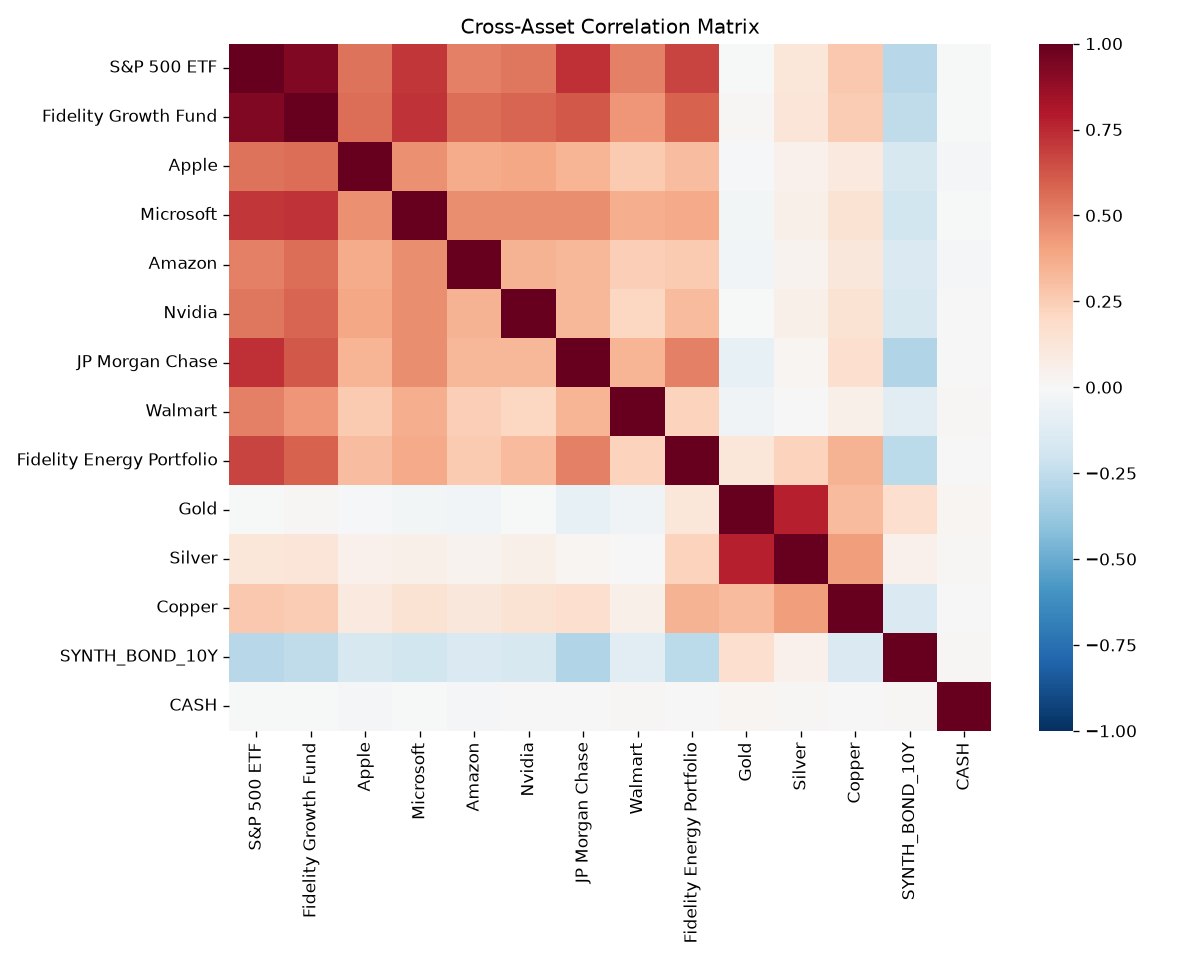
\includegraphics[width=\linewidth]{eda/correlation_matrix.png}
\end{minipage}\hfill
\begin{minipage}[t]{0.48\textwidth}
\centering
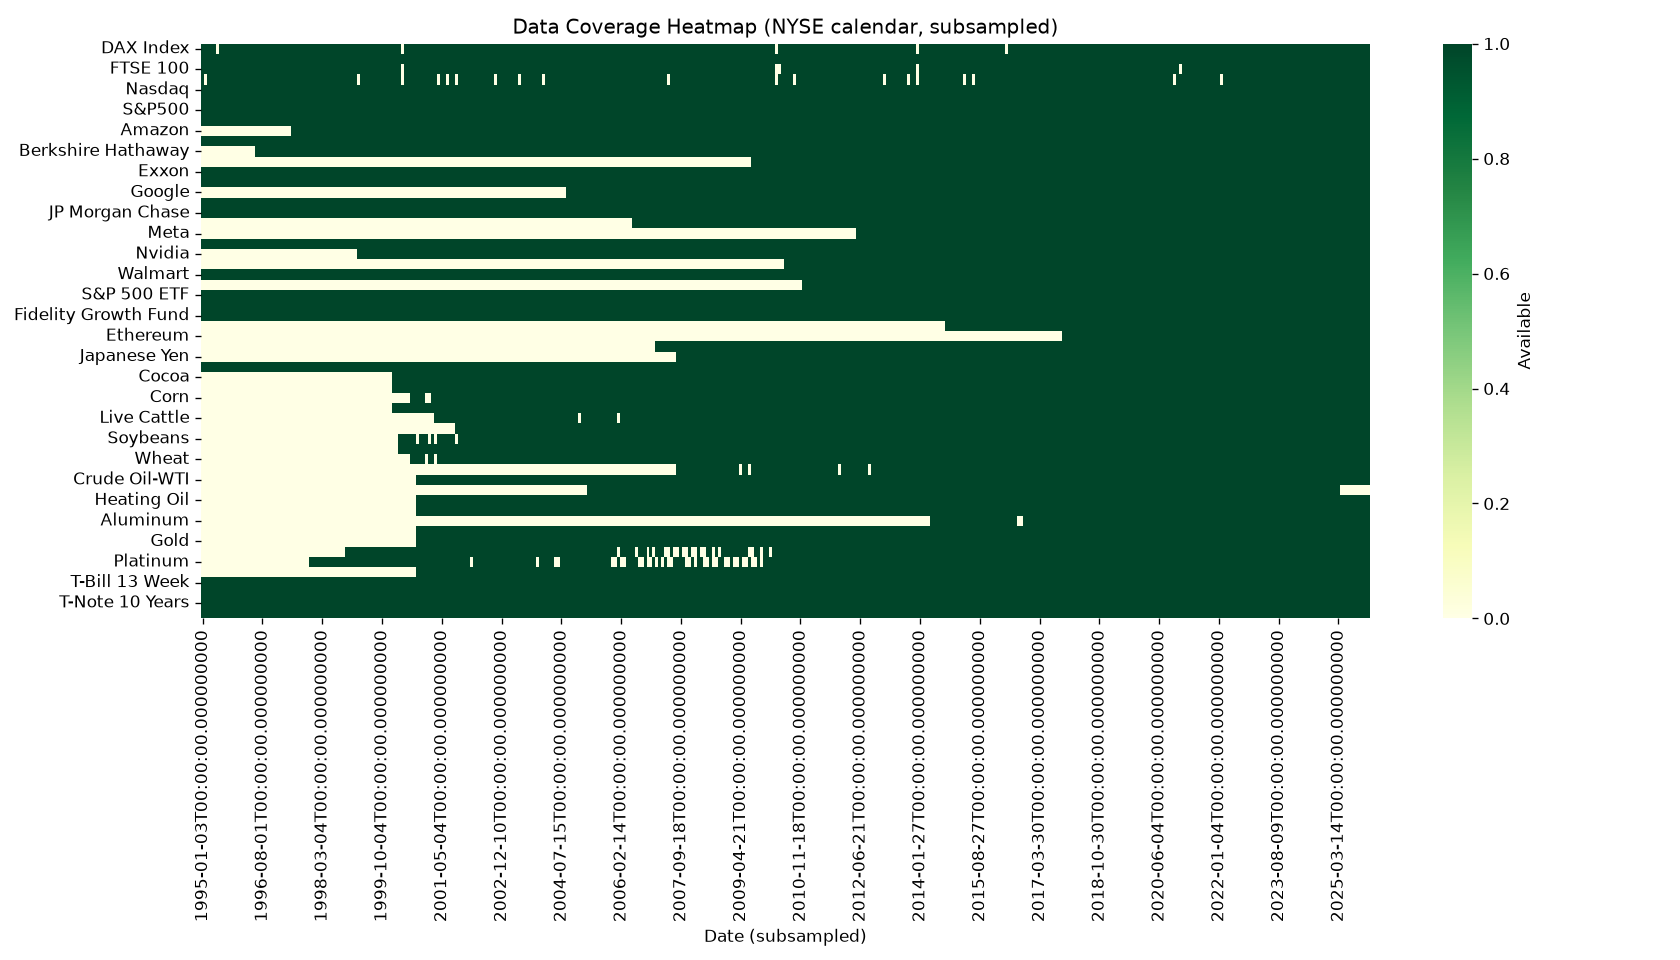
\includegraphics[width=\linewidth]{eda/coverage_heatmap.png}
\end{minipage}
\caption{\textbf{Left:} daily-return correlation matrix of the 14 investable assets over
2000--2025. The block structure is what makes diversification feasible and is precisely the
structure a mean-variance optimiser exploits: the nine equity-like instruments form a tightly
correlated cluster ($\rho \approx 0.4$--$0.9$), the three metals form a second, weaker cluster,
the synthetic 10-year bond is mildly \emph{negatively} correlated with equities, and cash is
uncorrelated with everything. \textbf{Right:} data-coverage heatmap over calendar time. Coverage
is the reason Universe~A starts in September 2000 rather than 1995---the metals series begin on
2000-08-30---and the reason Bitcoin and aluminium are quarantined into Universe~B.}
\label{fig:eda1}
\end{figure}

\begin{figure}[t]
\centering
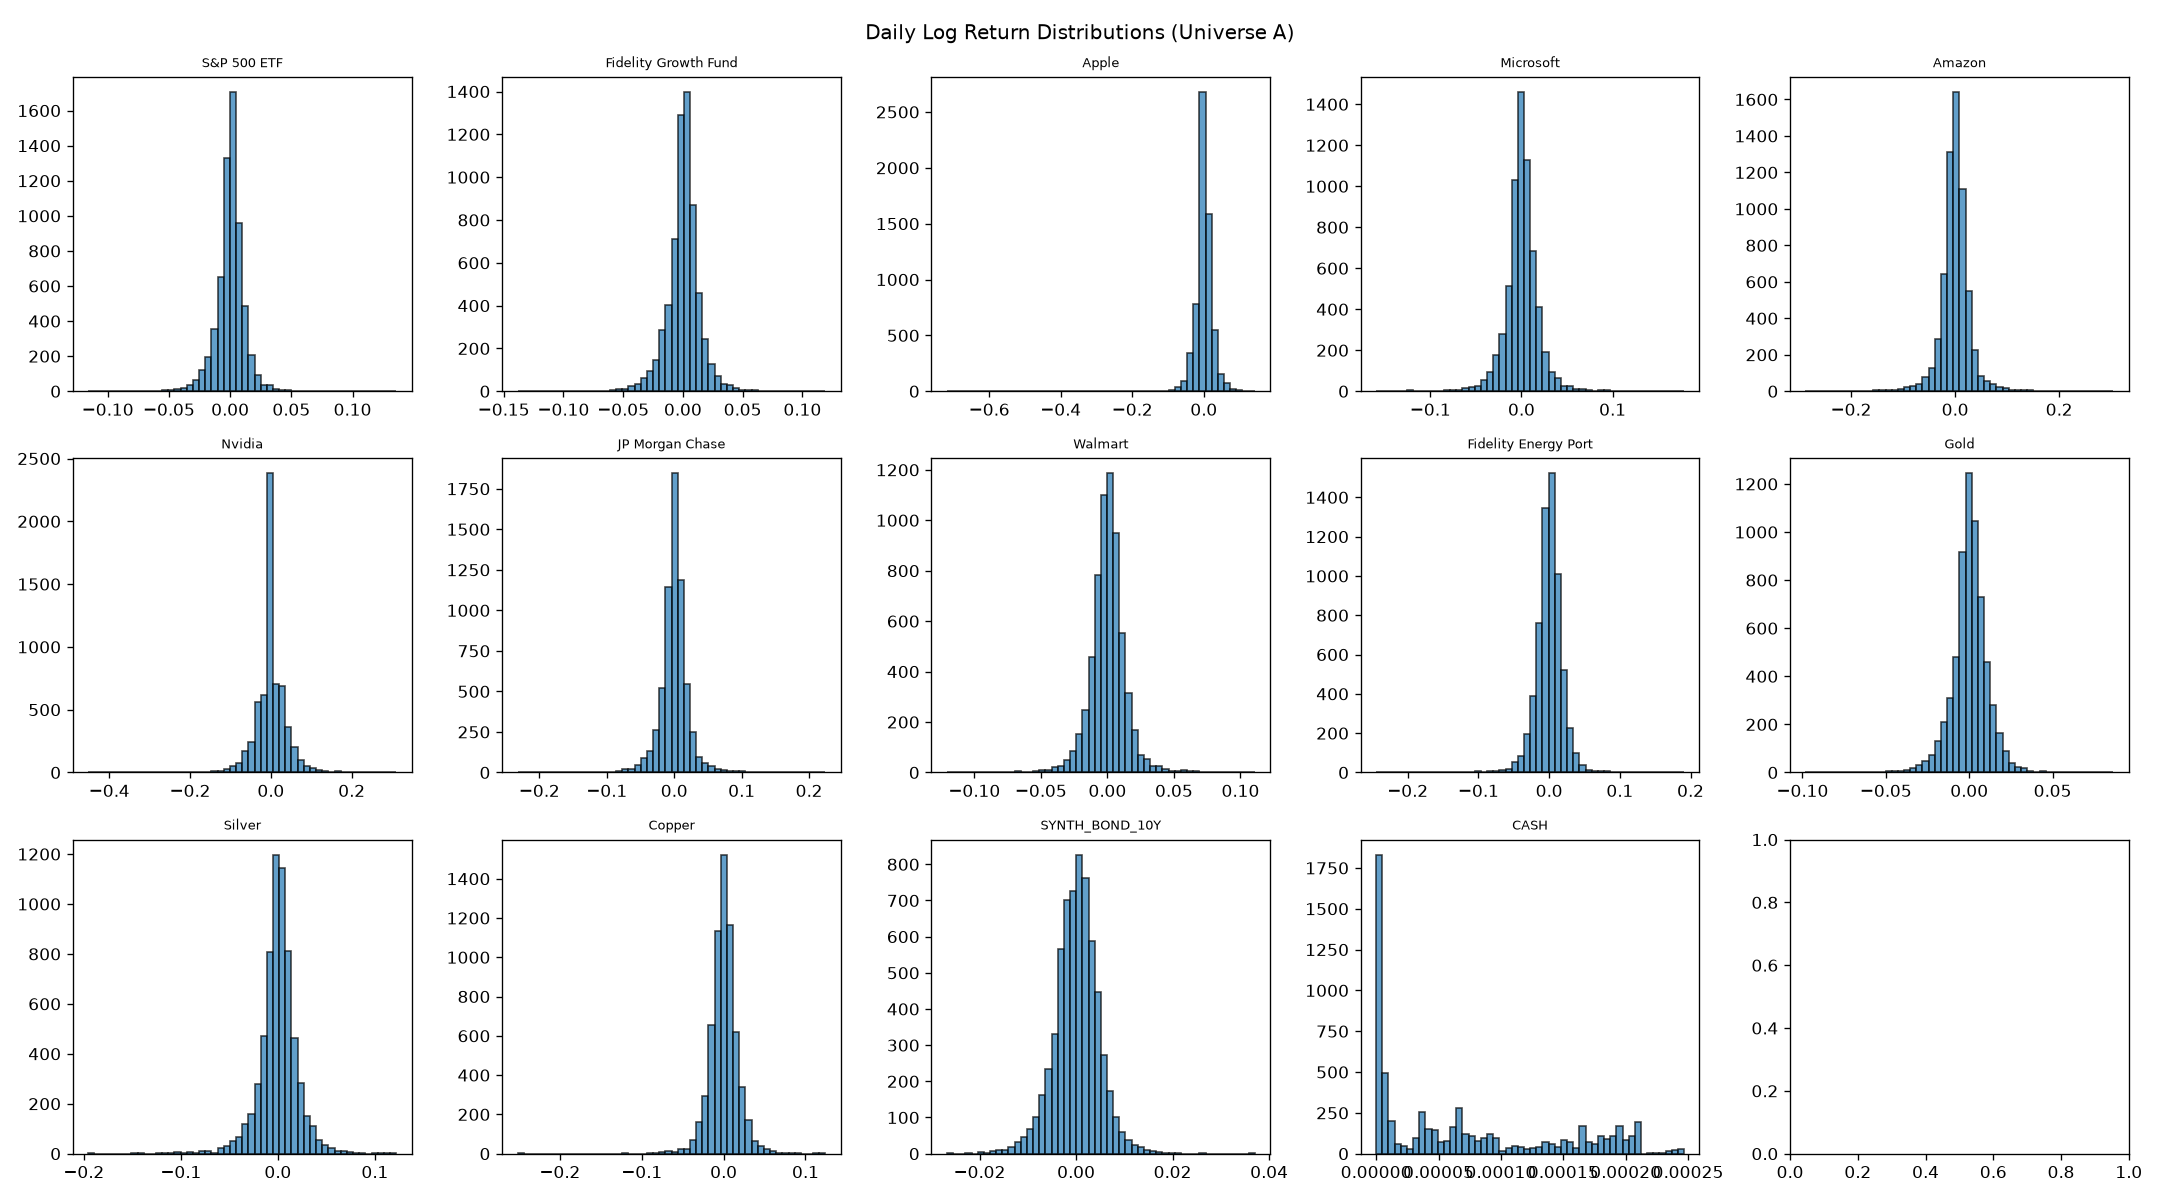
\includegraphics[width=0.95\textwidth]{eda/return_distributions.png}
\caption{Daily log-return histograms for all 14 investable assets, 2000--2025. Every equity and
metal series is leptokurtic with visible fat tails and occasional single-day moves beyond
$\pm 20\%$ (Apple, Nvidia, Amazon, the energy fund); the synthetic 10-year bond is much tighter;
and cash is a strictly non-negative, near-discrete series pinned to the T-bill yield and floored
at zero after 2020. Two consequences drive design choices elsewhere in the paper: the fat tails
mean a Gaussian Sharpe test is inadequate and motivate the block-bootstrap and Ledoit--Wolf
procedures of Section~\ref{sec:eval}, and the crash days make the raw $\ln(\cdot)$ reward
divergent, which is why the environment floors the net growth factor at
$\varepsilon = 10^{-8}$.}
\label{fig:eda2}
\end{figure}

\subsection{Tools / Models / Algorithms Used}
\label{sec:models}

The whole project is implemented from scratch in Python~3.12 with PyTorch~2.5 (CUDA~12.1),
NumPy, pandas, scikit-learn (for the Ledoit--Wolf covariance estimator) and matplotlib. We
deliberately did \emph{not} use FinRL, d3rlpy or stable-baselines3: the correctness
issues we discuss in Section~\ref{sec:bugs} are exactly the kind that a black-box library hides,
and the point of the study is to control the comparison. Training ran on a single NVIDIA GTX~1070
(8\,GB, Pascal).

\subsubsection{The allocation MDP}

We model daily rebalancing as a finite-horizon MDP
$\mathcal{M} = \langle \mathcal{S}, \mathcal{A}, P, R, \gamma, \rho_0, T_{\text{ep}}\rangle$
driven by an \emph{exogenous} price process: the agent chooses weights and pays turnover costs,
but cannot move prices. Let $y_t = (p_{1,t}/p_{1,t-1}, \dots, p_{N,t}/p_{N,t-1})^\top$ be the
vector of gross returns. The action is a long-only, fully-invested allocation on the simplex,
\begin{equation}
  a_t = w_t \in \Delta^{N-1} = \Big\{ w \in \mathbb{R}^N :\ w_i \ge 0,\ \textstyle\sum_{i=1}^{N} w_i = 1 \Big\},
\end{equation}
which forbids shorting and leverage; every model enforces this either with a softmax output
head or with a Euclidean projection onto $\Delta^{N-1}$. The state $s_t \in \mathbb{R}^{2580}$
is the standardised flattened feature window of Section~\ref{sec:data}. The reward is the net
logarithmic growth of the portfolio after a proportional cost $\mu$ on $L_1$ turnover,
\begin{equation}
  R_t \;=\; \ln\Big( \max\big\{\, a_t^\top y_t \;-\; \mu \textstyle\sum_{i=1}^{N} |a_{i,t} - a_{i,t-1}| ,\ \varepsilon \,\big\} \Big),
  \qquad \mu = 0.001,\ \varepsilon = 10^{-8},
  \label{eq:reward}
\end{equation}
so that maximising $\sum_t R_t$ maximises terminal wealth; the floor keeps $\ln$ defined on days
when costs would exceed gross growth. Return-to-Go is the undiscounted remaining reward,
\begin{equation}
  \hat{R}_t = \sum_{t'=t}^{T_{\text{ep}}-1} R_{t'}, \qquad \gamma = 1,
\end{equation}
which is exactly the quantity the Decision Transformer conditions on. Training episodes have
$T_{\text{ep}} = 252$ days (one trading year).

\paragraph{Behaviour policies and the offline buffer.}
Because there is no logged trading record to learn from, the offline dataset must be synthesised.
We roll out a mixture of 18 policies: six classical allocators (buy-and-hold, equal weight,
max-Sharpe mean-variance with a Ledoit--Wolf covariance estimate \cite{ledoit2004wellconditioned},
minimum-variance, inverse-volatility risk parity, and 60-day cross-sectional momentum), nine
Dirichlet-perturbed copies of mean-variance/momentum/equal-weight at concentrations
$\alpha \in \{5, 15, 50\}$, and three pure random Dirichlet policies at
$\alpha \in \{0.5, 1, 2\}$. The deliberate inclusion of bad and noisy policies is what makes
the dataset suitable for offline RL at all: a buffer containing only good behaviour cannot
teach a value-based method to distinguish good from bad, and it removes any opportunity for
DT to ``stitch'' high-return segments. Sampling 200 windows of 252 days from the training
range for each policy gives 3{,}600 episodes and roughly $8.2 \times 10^{5}$ usable
transitions. Trajectories are stored in a compact format in which all episodes index into a
single shared state matrix, which reduces the buffer from ${\sim}9.4$\,GB to ${\sim}65$\,MB
and lets the whole dataset live in GPU memory during training.

\subsubsection{Model 1: Decision Transformer}

\begin{figure}[t]
\centering
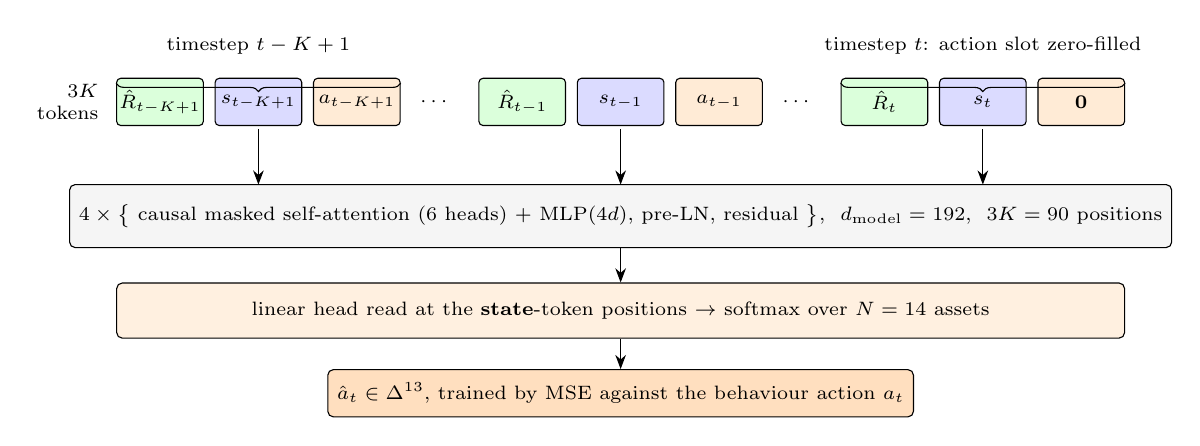
\begin{tikzpicture}[
  font=\scriptsize,
  tok/.style={draw, rounded corners=1.5pt, minimum width=11mm, minimum height=6mm,
              align=center, inner sep=1pt},
  rtg/.style={tok, fill=green!14}, st/.style={tok, fill=blue!14}, ac/.style={tok, fill=orange!16},
  blk/.style={draw, rounded corners=2pt, fill=gray!8, minimum width=128mm,
              minimum height=8mm, align=center},
  arr/.style={-{Stealth[length=1.8mm]}}
]
\def\yt{0}
\node[rtg] (r1) at (0.00,\yt) {$\hat{R}_{t-K+1}$};
\node[st]  (s1) at (1.25,\yt) {$s_{t-K+1}$};
\node[ac]  (a1) at (2.50,\yt) {$a_{t-K+1}$};
\node      (d1) at (3.50,\yt) {$\cdots$};
\node[rtg] (r2) at (4.60,\yt) {$\hat{R}_{t-1}$};
\node[st]  (s2) at (5.85,\yt) {$s_{t-1}$};
\node[ac]  (a2) at (7.10,\yt) {$a_{t-1}$};
\node      (d2) at (8.10,\yt) {$\cdots$};
\node[rtg] (r3) at (9.20,\yt) {$\hat{R}_{t}$};
\node[st]  (s3) at (10.45,\yt) {$s_{t}$};
\node[ac]  (a3) at (11.70,\yt) {$\mathbf{0}$};

\draw[decorate, decoration={brace, amplitude=3pt, raise=2pt}]
  (a1.north east) -- (r1.north west)
  node[midway, above=5pt, font=\scriptsize] {timestep $t-K+1$};
\draw[decorate, decoration={brace, amplitude=3pt, raise=2pt}]
  (a3.north east) -- (r3.north west)
  node[midway, above=5pt, font=\scriptsize] {timestep $t$: action slot zero-filled};

\node[blk] (b1) at (5.85,-1.45)
  {$4 \times \big\{$ causal masked self-attention (6 heads) $+$ MLP($4d$), pre-LN, residual $\big\}$,\ \
   $d_{\text{model}} = 192$, \ $3K = 90$ positions};
\node[blk, minimum height=7mm, fill=orange!12] (head) at (5.85,-2.65)
  {linear head read at the \textbf{state}-token positions $\rightarrow$ softmax over $N = 14$ assets};
\node[draw, rounded corners=2pt, fill=orange!25, minimum height=6mm] (out) at (5.85,-3.7)
  {$\hat{a}_t \in \Delta^{13}$, trained by MSE against the behaviour action $a_t$};

\foreach \x in {1.25, 5.85, 10.45} { \draw[arr] (\x,-0.35) -- (\x,-1.05); }
\draw[arr] (b1) -- (head);
\draw[arr] (head) -- (out);
\node[left=1mm of r1, align=right, font=\scriptsize] {$3K$\\ tokens};
\end{tikzpicture}
\caption{Decision Transformer architecture as implemented. Each timestep contributes three
tokens---Return-to-Go, state and action---so a context of $K=30$ timesteps becomes a
90-token sequence. A causal mask prevents any position from attending to the future, the
action head reads only the \emph{state}-token positions (so the prediction at step $t$ sees
$\hat{R}_t$ and $s_t$ but not $a_t$), and a softmax output enforces the simplex constraint
exactly. At inference the current-step action slot is zero-filled, since the causal mask
already hides it. Transformer BC is byte-for-byte this network with the Return-to-Go channel
zeroed, which makes it an exact control for the value of return conditioning.}
\label{fig:dt}
\end{figure}

The Decision Transformer \cite{chen2021decision} is our primary model
(Figure~\ref{fig:dt}). It interleaves three token types per timestep---the standardised
Return-to-Go scalar, the state, and the action---each passed through its own linear encoder
into a $d_{\text{model}}=192$ embedding, added to a learned positional embedding over the
$3K$ token slots, and processed by a 4-layer pre-LayerNorm causal transformer with 6 attention
heads. Predictions are read off the \emph{state}-token positions and passed through a softmax,
which enforces $a_t \in \Delta^{N-1}$ by construction rather than by projection. Training
minimises the mean squared error between the predicted allocation at the final context
position and the behaviour action recorded in the buffer. At evaluation time the RTG budget is
initialised to a chosen quantile of the training episodes' starting RTG, standardised with the
$(\mu_{\text{RTG}}, \sigma_{\text{RTG}}) = (-0.0023, 0.1394)$ statistics computed on the
training set, decremented by each realised log reward, and reset every 252 steps so that a
six-year rollout stays in the range of remaining-return values the model actually saw during
training. We chose DT because it is the method under test: it is the only model here that can,
in principle, be \emph{asked} for a return level at inference time, and the entire
experimental design is built around checking whether that request has any effect.

\subsubsection{Model 2: Transformer Behaviour Cloning (the RTG control)}

Transformer BC is the same network with the Return-to-Go channel zeroed, so it has the same
$2{,}298{,}638$ parameters, the same optimiser, the same batches and the same seeds as DT, and
differs \emph{only} in whether it can see the return target. This is the single most important
baseline in the paper. Any gap between DT and BC is attributable to return conditioning and to
nothing else; conversely, if DT $\approx$ BC then the transformer is merely imitating the
behaviour mixture and the ``decision'' half of Decision Transformer is inert. We are not aware
of a portfolio-allocation study that reports this control, which is one reason we consider the
comparison worth publishing even though its outcome is negative.

\subsubsection{Models 3--5: offline RL (TD3+BC, IQL, CQL)}

\begin{figure}[t]
\centering
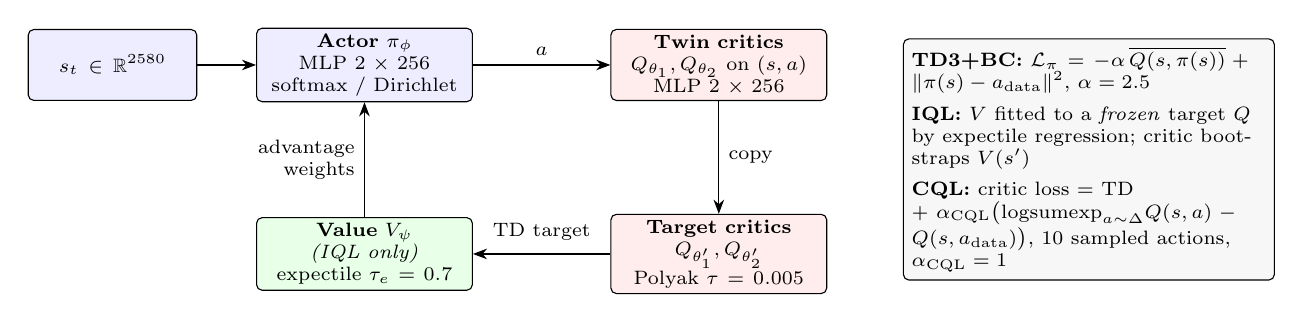
\begin{tikzpicture}[
  font=\scriptsize,
  net/.style={draw, rounded corners=2pt, align=center, minimum height=9mm,
              text width=26mm, inner sep=2pt, fill=blue!7},
  cri/.style={net, fill=red!7}, val/.style={net, fill=green!9},
  arr/.style={-{Stealth[length=1.8mm]}}
]
\node[net, text width=20mm] (s)      at (0.0,  0.0) {$s_t \in \mathbb{R}^{2580}$};
\node[net]                  (actor)  at (3.2,  0.0) {\textbf{Actor} $\pi_\phi$\\ MLP $2\times256$\\ softmax / Dirichlet};
\node[cri]                  (critic) at (7.7,  0.0) {\textbf{Twin critics}\\ $Q_{\theta_1}, Q_{\theta_2}$ on $(s,a)$\\ MLP $2\times256$};
\node[cri]                  (target) at (7.7, -2.4) {\textbf{Target critics}\\ $Q_{\theta'_1}, Q_{\theta'_2}$\\ Polyak $\tau = 0.005$};
\node[val]                  (value)  at (3.2, -2.4) {\textbf{Value} $V_\psi$\\ \emph{(IQL only)}\\ expectile $\tau_e = 0.7$};

\draw[arr] (s)      -- (actor);
\draw[arr] (actor)  -- node[above, font=\scriptsize] {$a$} (critic);
\draw[arr] (critic) -- node[right, font=\scriptsize] {copy} (target);
\draw[arr] (target) -- node[above=0.5mm, font=\scriptsize] {TD target} (value);
\draw[arr] (value)  -- node[left, font=\scriptsize, align=right]
  {advantage\\ weights} (actor);

\node[draw, rounded corners=2pt, fill=gray!6, align=left, text width=45mm,
      inner sep=3pt, font=\scriptsize] at (12.4, -1.2)
  {\textbf{TD3+BC:} $\mathcal{L}_\pi = -\alpha\,\overline{Q(s,\pi(s))} + \lVert \pi(s) - a_{\text{data}}\rVert^2$, $\alpha = 2.5$\\[1.2mm]
   \textbf{IQL:} $V$ fitted to a \emph{frozen} target $Q$ by expectile regression; critic bootstraps $V(s')$\\[1.2mm]
   \textbf{CQL:} critic loss $=$ TD $+\ \alpha_{\text{CQL}}\big(\mathrm{logsumexp}_{a\sim\Delta} Q(s,a) - Q(s,a_{\text{data}})\big)$, 10 sampled actions, $\alpha_{\text{CQL}} = 1$};
\end{tikzpicture}
\caption{Shared actor--critic skeleton of the three offline RL baselines and the point at which
each algorithm departs from it. All three use two-hidden-layer MLPs of width 256, twin critics
with Polyak-averaged targets ($\tau=0.005$), $\gamma = 0.99$, Adam at $3\times10^{-4}$, and a
simplex projection on the actor output. The shared bootstrap target is
$r + \gamma(1-d)\min_i Q_{\theta'_i}(s', \pi(s'))$, with the done flag $d$ cutting the bootstrap
at an episode boundary. TD3+BC \cite{fujimoto2021minimalist} anchors the
policy to the data with an explicit BC term; IQL \cite{kostrikov2022offline} never queries
out-of-distribution actions at all, fitting an expectile value function instead; CQL
\cite{kumar2020conservative} pushes down $Q$-values on actions sampled from the simplex
relative to the dataset action.}
\label{fig:offlinerl}
\end{figure}

These three represent the value-based branch of offline RL and are included because they are
the methods DT is supposed to replace (Figure~\ref{fig:offlinerl}). \textbf{TD3+BC}
\cite{fujimoto2021minimalist} is TD3 \cite{fujimoto2018addressing} plus a behaviour-cloning
regulariser with weight $\alpha=2.5$; we chose it because it is the strongest
``one-line-change'' offline baseline in the literature and therefore the fairest cheap
comparison. \textbf{IQL} \cite{kostrikov2022offline} fits an expectile ($\tau_e = 0.7$) value
function to a frozen target critic and trains the actor by advantage-weighted regression; we
chose it because it never evaluates $Q$ at actions outside the data, which is the most
conservative possible response to the distribution shift our noisy behaviour mixture creates.
\textbf{CQL} \cite{kumar2020conservative} adds a conservative penalty with weight
$\alpha_{\text{CQL}}=1$ computed as a log-sum-exp over ten actions sampled from the simplex per
state, i.e.\ the CQL(H) variant; we chose it as the pessimism-based counterpoint to IQL's
avoidance-based approach. All three use $\gamma = 0.99$, Polyak targets with $\tau = 0.005$,
Adam at $3\times 10^{-4}$, and two-hidden-layer MLPs of width 256 for both actor and critics.

\subsubsection{Models 6--8: online RL reference points (PPO, SAC, A2C)}

PPO \cite{schulman2017proximal}, SAC \cite{haarnoja2018soft} and A2C
\cite{mnih2016asynchronous} are included because they are what the applied
literature actually uses for portfolio RL \cite{yang2020deep,liu2021finrl}, and a reader will
want to see them. We must be explicit about a caveat: in our pipeline they perform single-step
updates over the same \emph{offline} buffer rather than interacting with a live environment,
because the whole premise of the study is that online interaction is unavailable. They are
therefore reference points, not a fair online comparison, and we never claim otherwise. PPO
and SAC use a Dirichlet actor (concentration $\mathrm{softplus}(f_\phi(s)) + 1$) and act with
the Dirichlet mean; A2C uses a softmax actor.

\subsubsection{Classical baselines}

Six parameter-free allocators provide the bar the learners must clear:
\textbf{buy-and-hold} and \textbf{equal weight} (both emit $\mathbf{1}/N$ daily---under a
target-referenced turnover model these coincide);
\textbf{mean-variance} (max-Sharpe Markowitz \cite{markowitz1952portfolio} on a 252-day window
with a Ledoit--Wolf shrunk covariance \cite{ledoit2004wellconditioned}, solved by 200 projected
gradient steps on the simplex);
\textbf{minimum-variance} (same solver, variance objective);
\textbf{risk parity} (inverse 60-day volatility);
and \textbf{momentum} (equal weight over the top $\lfloor N/3 \rfloor = 4$ assets by 60-day
trailing return).

\subsubsection{Hyperparameters}

Table~\ref{tab:hparams} lists every hyperparameter. The transformer shape
($K=30$, $d_{\text{model}}=192$, 4 layers, 6 heads) was chosen to fit the 8\,GB GTX~1070 while
leaving room for a GPU-resident replay buffer, and $K$ is ablated in
Section~\ref{sec:ablation-k}. The optimiser is AdamW \cite{loshchilov2019decoupled} at
$10^{-4}$ with weight decay $10^{-4}$ and a cosine schedule over 50 epochs, with gradient-norm
clipping at $1.0$; these are the Decision Transformer paper's settings scaled down for our
model size. Batch size 256 was selected empirically: measured throughput on this GPU plateaus
near $1{,}300$ samples/s for every batch size from 128 to 1024, so larger batches buy only
VRAM. Mixed precision is deliberately disabled---the Pascal GP104 chip has no tensor cores and
runs fp16 at roughly $1/64$ of fp32 throughput, so AMP would slow training down. Finally,
\texttt{steps\_per\_epoch} is capped at 200: a full pass over the buffer is 3{,}189 steps, which
would make the five-seed sweep a ${\sim}87$-hour job, whereas $50 \times 200$ steps still covers
about three full passes and fits in an overnight window.

\begin{table}[t]
\centering
\caption{Hyperparameters. All learned models share the training budget, the seed set and the
batch size, so differences between them are attributable to the algorithm rather than to
tuning effort.}
\label{tab:hparams}
\small
\begin{tabular}{llll}
\toprule
\textbf{Group} & \textbf{Hyperparameter} & \textbf{Value} & \textbf{Why} \\
\midrule
\multirow{4}{*}{Environment}
 & transaction cost $\mu$ & $0.001$ (10\,bp) & retail-realistic; ablated over $\{0,5,10,25\}$\,bp \\
 & reward floor $\varepsilon$ & $10^{-8}$ & keeps $\ln(\cdot)$ finite on crash days \\
 & episode length $T_{\text{ep}}$ & 252 & one trading year; also the RTG reset horizon \\
 & episode stride & 21 & one month; decorrelates sampled windows \\
\midrule
\multirow{6}{*}{Transformer}
 & context length $K$ & 30 & $90$ tokens; ablated over $\{10,20,30,50\}$ \\
 & $d_{\text{model}}$ / layers / heads & $192$ / $4$ / $6$ & 2.30\,M params, fits 8\,GB with the buffer resident \\
 & dropout & $0.1$ & mild regularisation; train/val curves stay together \\
 & optimiser & AdamW, cosine & \cite{loshchilov2019decoupled}; DT paper's choice \\
 & learning rate / weight decay & $10^{-4}$ / $10^{-4}$ & stable at this model size \\
 & gradient clip & $1.0$ & prevents rare large-loss spikes \\
\midrule
\multirow{5}{*}{RL agents}
 & hidden width / depth & $256$ / $2$ & matched across TD3+BC, IQL, CQL, PPO, SAC, A2C \\
 & discount $\gamma$ & $0.99$ & standard; DT uses $\gamma=1$ for RTG \\
 & Polyak $\tau$ & $0.005$ & standard TD3 setting \\
 & TD3+BC $\alpha$ / IQL expectile & $2.5$ / $0.7$ & paper defaults \\
 & CQL $\alpha_{\text{CQL}}$ / \#\,actions & $1.0$ / $10$ & CQL(H) over sampled simplex actions \\
\midrule
\multirow{4}{*}{Training}
 & seeds & $\{42,123,456,789,1011\}$ & 5 runs per model; we report mean $\pm$ std \\
 & epochs $\times$ steps/epoch & $50 \times 200$ & ${\sim}3$ passes over 816k transitions \\
 & batch size & $256$ & throughput plateaus at ${\sim}1300$ samples/s \\
 & mixed precision & disabled & Pascal fp16 is ${\sim}1/64$ of fp32 throughput \\
\midrule
Inference & target RTG quantile & $0.90$ & of training-episode starting RTG; ablated \\
\bottomrule
\end{tabular}
\end{table}

\subsection{Performance Evaluation}
\label{sec:eval}

\paragraph{Data partition.}
The split is strictly chronological, never random, because randomly shuffled financial data
leaks the future into the past through overlapping feature windows. The
\textbf{training} period is 2000-09-01 to 2016-12-31, the \textbf{validation} period is
2017-01-01 to 2019-12-31, and the \textbf{test} period is 2020-01-01 to 2025-12-30
(1{,}507 trading days). Feature standardisation statistics, behaviour-policy rollouts and all
offline episodes come from the training period alone. Validation is used only for model
selection---the checkpoint with the lowest validation action MSE is the one that gets
backtested---and is never backtested for reporting. Beyond this fixed holdout we also run a
\textbf{walk-forward} evaluation over six two-year blocks (2014--15, 2016--17, 2018--19,
2020--21, 2022--23, 2024--25); the first two begin before the training cutoff and are flagged
in-sample, and we report them only as a sanity check.

\paragraph{Error function.}
The training objective for DT and BC is the mean squared error between the predicted allocation
and the behaviour action,
$\mathcal{L}(\theta) = \mathbb{E}_{\tau \sim \mathcal{D}}\big[\lVert a_t - \hat{f}_\theta(\hat{R}_{t-K+1:t}, s_{t-K+1:t}, a_{t-K+1:t-1})\rVert_2^2\big]$,
evaluated at the last context position. The RL agents instead minimise their algorithm-specific
temporal-difference and actor losses over the same transitions. Note that a low MSE means
faithful \emph{imitation}, not good \emph{allocation}---this distinction turns out to matter,
and Section~\ref{sec:ablation-k} shows the two moving in opposite directions.

\paragraph{Financial metrics.}
Every strategy is scored on the same log-return series with the same code: cumulative return,
CAGR, annualised volatility, \textbf{Sharpe ratio} \cite{sharpe1994sharpe} (our headline
metric, computed against a 2\% annual risk-free rate on a 252-day year), Sortino ratio,
maximum drawdown, Calmar ratio, 95\% VaR and CVaR, and mean daily $L_1$ turnover. We lead with
Sharpe rather than return because with a simplex action space any strategy can raise its return
by concentrating into whatever rallied, and Sharpe is what penalises that.

\paragraph{Statistical testing.}
Because daily returns are fat-tailed (Figure~\ref{fig:eda2}) and serially dependent, we do not
test Sharpe differences with a Gaussian assumption. We report (i) 95\% confidence intervals for
the Sharpe difference against buy-and-hold from a circular block bootstrap (block length 20,
1{,}000 replicates) in the spirit of \cite{politis1994stationary}, (ii) the Ledoit--Wolf robust
Sharpe-difference test \cite{ledoit2008robust}, and (iii) the deflated Sharpe ratio
\cite{bailey2014deflated} with $n_{\text{trials}} = 46$, the total number of strategy variants
evaluated. Reporting a multiple-testing correction is essential here: a study that trains 40
checkpoints and reports the best one is guaranteed to find something.

\section{Experimental Analysis}

Code, configuration and all result tables are available at\\
\url{https://github.com/ShojebBhuiyan/Decision-Transformer-for-Sequential-Portfolio-Allocation-using-Offline-Reinforcement-Learning}.
The full pipeline is reproducible with \texttt{python main.py --stage all}; the ablation sweeps
of Section~\ref{sec:ablations} are produced by \texttt{scripts/run\_paper\_ablations.py} and the
figures by \texttt{scripts/run\_paper\_figures.py}. A suite of 58 unit tests covers the
correctness safeguards (simplex validity, hand-computed rewards, no-lookahead features, the RTG
recursion, split-boundary leakage, and the RL fixes of Section~\ref{sec:bugs}).

\subsection{Convergence}

\begin{figure}[t]
\centering
\includegraphics[width=\textwidth]{paper/convergence.png}
\caption{Training and validation action-MSE for the Decision Transformer (left) and the
architecturally identical RTG-free control (right). Solid lines are the mean over the five
seeds $\{42,123,456,789,1011\}$; shaded bands span the seed-wise minimum and maximum. Both
models fall steeply for roughly 10 epochs and then flatten, converging to
$\approx 3.2\times10^{-3}$ by epoch 50, and the validation curve tracks the training curve for
the whole run with no upward turn---i.e.\ neither model overfits the offline buffer, and the
50-epoch budget is sufficient. Two observations matter for the rest of the paper. First, the
two panels are nearly superimposable: adding the Return-to-Go channel lowers the best
validation MSE by only $1.2\times10^{-5}$ (a $0.4\%$ relative improvement), the first sign that
the conditioning signal carries almost no usable information. Second,
the seed spread on the loss is far narrower than the seed spread we later see on backtest
Sharpe ($\pm 0.13$), which means the variance in Table~\ref{tab:learned} comes from how small
weight differences compound over a 1{,}507-day rollout, not from unstable optimisation.}
\label{fig:convergence}
\end{figure}

Figure~\ref{fig:convergence} shows the convergence of the two transformer models. Both
converge cleanly and identically. Averaged over seeds, DT ends at a training MSE of
$3.245\times10^{-3}$ and a best validation MSE of $3.245\times10^{-3}$; BC ends at
$3.263\times10^{-3}$ and $3.257\times10^{-3}$. Validation loss reaches its minimum at epoch 47--50
in every one of the ten runs, so no run was stopped early by the checkpoint-selection rule and
none diverged. Since the validation curve never separates from the training curve, the
generalisation gap on the \emph{imitation} task is essentially zero---which, as the backtests
will show, does not translate into generalisation on the \emph{allocation} task.

\subsection{Classical baselines on the 2020--2025 holdout}

\begin{table}[t]
\centering
\caption{Universe~A, held-out test period 2020-01-01 to 2025-12-30 (1{,}507 trading days),
$\mu = 10$\,bp. Turnover is mean daily $L_1$ turnover. Buy-and-hold and equal weight are
identical under a target-referenced turnover model and are reported once.}
\label{tab:classical}
\small
\begin{tabular}{lrrrrrrr}
\toprule
Strategy & Cum.\ ret. & CAGR & Vol. & \textbf{Sharpe} & Sortino & Max DD & Turnover \\
\midrule
Buy-and-hold / $1/N$ & $2.569$ & $0.237$ & $0.172$ & $\mathbf{1.118}$ & $1.379$ & $-0.233$ & ${\sim}0$ \\
Mean-variance        & $2.647$ & $0.242$ & $0.176$ & $1.116$ & $1.393$ & $-0.233$ & $0.007$ \\
Minimum-variance     & $2.527$ & $0.235$ & $0.171$ & $1.116$ & $1.372$ & $-0.233$ & $0.0002$ \\
Momentum             & $3.199$ & $\mathbf{0.271}$ & $0.226$ & $0.973$ & $1.311$ & $-0.320$ & $0.151$ \\
Risk parity          & $0.034$ & $0.006$ & $0.081$ & $-0.178$ & $-0.145$ & $-0.233$ & $0.001$ \\
\bottomrule
\end{tabular}
\end{table}

Table~\ref{tab:classical} establishes the bar. Equal weight earns a Sharpe of $1.118$ with a
CAGR of $23.7\%$ and a maximum drawdown of $-23.3\%$, and neither Markowitz optimisation nor
minimum-variance improves on it in any statistically meaningful way: their Sharpe differences
are $-0.0028$ with bootstrap CIs of $[-0.066, 0.052]$ and $[-0.011, 0.007]$ and Ledoit--Wolf
$p$-values of $0.91$ and $0.97$. This is the classic ``$1/N$ is hard to beat'' result
\cite{demiguel2009optimal} reproduced on our universe, and it is why the study needs
significance testing rather than a leaderboard. Momentum produces the highest raw growth
($27.1\%$ CAGR) but pays for it with $22.6\%$ volatility, a $-32.0\%$ drawdown and $15.1\%$
mean daily turnover, so its Sharpe is $0.973$---worse than doing nothing, with $p = 0.0002$.
Risk parity fails outright ($0.6\%$ CAGR, Sharpe $-0.178$): inverse-volatility weighting pours
capital into the cash and bond sleeve, which is precisely the wrong place to be during the
2020--2025 equity run.

\subsection{Learned allocators}
\label{sec:learned-hold}

\begin{table}[t]
\centering
\caption{Universe~A test period, learned allocators: mean $\pm$ standard deviation across the
five seeds. Every row is a backtest of a trained checkpoint through the same environment used
for Table~\ref{tab:classical}. The buy-and-hold reference line is repeated for convenience.
$^\dagger$PPO's Dirichlet mean collapses to $\mathbf{1}/N$ on all five seeds, so it reproduces
buy-and-hold exactly (zero variance) by degenerating, not by allocating.}
\label{tab:learned}
\small
\begin{tabular}{lrrrrr}
\toprule
Model & CAGR & Volatility & \textbf{Sharpe} & Max DD & Turnover \\
\midrule
\emph{Buy-and-hold (reference)} & $0.237$ & $0.172$ & $1.118$ & $-0.233$ & ${\sim}0$ \\
\midrule
PPO$^\dagger$ (online ref.) & $0.237 \pm 0.000$ & $0.172$ & $1.118 \pm 0.000$ & $-0.233$ & ${\sim}0$ \\
SAC (online ref.)           & $0.222 \pm 0.029$ & $0.175$ & $1.039 \pm 0.160$ & $-0.248 \pm 0.044$ & $0.058$ \\
Transformer BC              & $0.219 \pm 0.009$ & $0.184$ & $0.976 \pm 0.106$ & $-0.267 \pm 0.048$ & $0.059$ \\
\textbf{Decision Transformer} & $0.215 \pm 0.011$ & $0.183$ & $0.966 \pm 0.133$ & $-0.272 \pm 0.062$ & $0.061$ \\
IQL                         & $0.196 \pm 0.035$ & $0.199$ & $0.818 \pm 0.204$ & $-0.303 \pm 0.025$ & $0.127$ \\
CQL                         & $\mathbf{0.343 \pm 0.117}$ & $0.346$ & $0.781 \pm 0.214$ & $-0.499 \pm 0.098$ & $0.195$ \\
TD3+BC                      & $0.190 \pm 0.060$ & $0.238$ & $0.660 \pm 0.261$ & $-0.351 \pm 0.033$ & $0.135$ \\
A2C (online ref.)           & $-0.014 \pm 0.113$ & $0.307$ & $-0.127 \pm 0.378$ & $-0.539 \pm 0.165$ & $1.139$ \\
\bottomrule
\end{tabular}
\end{table}

Table~\ref{tab:learned} is the central result, and it is negative: \textbf{no learned allocator
beats cost-aware equal weight on Sharpe}. The ordering is itself informative. PPO ties the
baseline exactly, but only because its Dirichlet concentration parameters collapse so that the
mean action is $\mathbf{1}/N$ on every seed---it is not allocating, it is abstaining, and the
zero standard deviation is the tell. SAC is the best genuinely active learner
($1.039 \pm 0.160$) and still trails. The Decision Transformer reaches $0.966 \pm 0.133$
against its RTG-free control's $0.976 \pm 0.106$: a gap of $-0.010$ Sharpe, an order of
magnitude smaller than the seed-to-seed spread of either model. The value-based offline methods
are clearly worse: IQL $0.818$, CQL $0.781$, TD3+BC $0.660$, all with much higher turnover
($12.7$--$19.5\%$ daily) and deeper drawdowns. CQL deserves a separate note because it is the
one row where a learned method looks impressive on the wrong axis: its mean CAGR of $34.3\%$ is
the highest number anywhere in this paper, but it is bought with $34.6\%$ volatility and a
$-49.9\%$ maximum drawdown, i.e.\ CQL's conservatism penalty pushes it into a few concentrated
bets that happened to work in this particular window. A2C is unusable, with mean daily turnover
above $1.0$ (it rewrites the entire portfolio every day) and negative CAGR.

One caveat on the transformer rows: their turnover is bimodal across seeds, not merely noisy.
Seeds 123, 456, 789 and 1011 all produce ${\sim}4.3\%$ mean daily turnover and Sharpe
$0.95$--$1.09$, while seed 42 produces $13.6\%$ (DT) and $12.3\%$ (BC) and Sharpe $0.75$/$0.81$.
The mode is a property of the \emph{seed}, not of the architecture---the same seed puts DT and
BC in the same mode---so the $0.061$ and $0.059$ turnover figures in Table~\ref{tab:learned} are
averages over two distinct behaviours rather than descriptions of a typical run. We return to
this in Section~\ref{sec:ablation-k}, where it limits what the context-length sweep can
establish.

\begin{figure}[t]
\centering
\includegraphics[width=\textwidth]{paper/equity_curves.png}
\caption{Cumulative wealth on the held-out window (log scale, initial capital $=1$,
$\mu = 10$\,bp). DT and BC are shown at seed 456, the median-Sharpe run; seed 42 is the
high-turnover outlier discussed in Section~\ref{sec:learned-hold}, and plotting it would
misrepresent a typical rollout. The visual story matches
Tables~\ref{tab:classical}--\ref{tab:learned}: buy-and-hold and mean-variance are
indistinguishable; momentum leads throughout on level but with visibly larger swings, including
a sharper 2022 drawdown; and DT and BC track the market closely while sitting persistently
\emph{below} it, the gap opening in the March 2020 crash and never closing. Risk parity
flatlines just above its starting capital for all six years. BC (dashed black) is drawn over DT
(red) because the two wealth paths are otherwise indistinguishable---the clearest single
illustration that return conditioning changes almost nothing.}
\label{fig:equity}
\end{figure}

Figure~\ref{fig:equity} shows the same result as wealth paths. The learned transformers do not
fail catastrophically---they track the market, which is what a behaviour-cloned policy over a
mixture dominated by sensible allocators should do---but they shed a few percent of terminal
wealth to turnover and to small timing errors, with the gap opening in the March 2020 crash and
never closing.

\subsection{What the learned allocators actually hold}

\begin{table}[h]
\centering
\caption{Mean allocation held over the test window, summarised by the Herfindahl--Hirschman
index $\mathrm{HHI} = \sum_i \bar{w}_i^2$, which equals $1/N = 0.0714$ for a perfectly uniform
book and $1$ for a single-asset book. Every learned row aggregates all five seeds; the bracketed
range is the seed minimum and maximum. This table explains the Sharpe ordering of
Table~\ref{tab:learned} better than any training metric does.}
\label{tab:concentration}
\small
\begin{tabular}{lccrl}
\toprule
Model & HHI (mean [min, max]) & Max mean & Turn- & What the book looks like \\
      &                       & weight   & over  & \\
\midrule
Equal weight ($1/N$) & $0.0714$ & $0.071$ & $\sim 0$ & uniform by construction \\
PPO    & $0.0714$ $[0.0714, 0.0714]$ & $0.071$ & $\sim 0$ & uniform on every seed \\
SAC    & $0.0732$ $[0.0723, 0.0741]$ & $0.097$ & $0.058$ & near-uniform; tilt varies by seed \\
BC     & $0.0742$ $[0.0715, 0.0846]$ & $0.090$ & $0.059$ & $1/N$ $+$ noise on 4 of 5 seeds \\
DT     & $0.0742$ $[0.0715, 0.0846]$ & $0.090$ & $0.061$ & $1/N$ $+$ noise on 4 of 5 seeds \\
IQL    & $0.0843$ $[0.0816, 0.0871]$ & $0.160$ & $0.127$ & cash-heavy \\
TD3+BC & $0.0865$ $[0.0820, 0.0932]$ & $0.152$ & $0.135$ & Nvidia / Apple / cash \\
A2C    & $0.1196$ $[0.1050, 0.1303]$ & $0.207$ & $1.139$ & cash $+$ megacaps, rewritten daily \\
CQL    & $0.2321$ $[0.2019, 0.2826]$ & $0.321$ & $0.195$ & Nvidia, Amazon, Apple on \emph{every} seed \\
\bottomrule
\end{tabular}
\end{table}

Aggregate performance metrics say what happened; Table~\ref{tab:concentration} says why. Four
readings stand out.

\textbf{PPO's collapse is exact.} Its HHI equals $1/14$ on all five seeds and its largest mean
weight is $0.0714$, so the ``tie'' with buy-and-hold in Table~\ref{tab:learned} is arithmetic
identity, not a coincidence of performance.

\textbf{DT and BC do not merely track equal weight---on four of five seeds they \emph{are} equal
weight plus noise.} At seeds 123, 456, 789 and 1011 their HHI is $0.0715$ against a uniform
$0.0714$, the largest mean weight is $7.5$--$7.9\%$ against a uniform $7.1\%$, and the three
largest holdings are effectively arbitrary: Walmart and silver at one seed, JP~Morgan and cash at
another, Nvidia and Microsoft at a third, with nothing above eight percent anywhere. Only the
fifth seed---the high-turnover run of Section~\ref{sec:learned-hold}---holds a real
megacap-growth tilt ($\mathrm{HHI} = 0.085$, Nvidia at $14\%$). The typical outcome of training a
Decision Transformer on this buffer is therefore a policy that reproduces the baseline's
allocation and then pays $4.3\%$ daily turnover to keep re-deriving it, which is precisely the
cost drag that Section~\ref{sec:ablation-cost} isolates. DT and BC are also indistinguishable
seed by seed, agreeing to the fourth decimal of HHI---a third independent confirmation of the
RTG result, after the loss curves and the Sharpe comparison.

\textbf{SAC scores best among the active learners because it deviates least}
($\mathrm{HHI} = 0.073$, largest mean weight under $10\%$). Its tilt is not even consistent
across seeds---copper and gold at one, the energy fund and silver at another---which is another
way of saying it has not learned a view.

\textbf{CQL is not being conservative at all.} Its HHI averages $0.232$---more than three times
uniform---and reaches $0.283$ at seed 789, where a single position averages $42\%$ of the book.
The concentration is systematic rather than random: on every one of the five seeds the three
largest holdings are Nvidia, Amazon and Apple, together $63$--$84\%$ of capital. Its $34.3\%$
CAGR and $-49.9\%$ maximum drawdown are one repeated bet on the 2020--2025 technology rally, not
evidence that pessimistic offline RL extracts a better policy. Universe~B makes the point
unmistakable: CQL's average book there is $80.2\%$ Nvidia and $13.2\%$ Bitcoin.

\subsection{Statistical significance}

\begin{table}[t]
\centering
\caption{Significance of each learned model's Sharpe against buy-and-hold on the test window.
``CI excludes 0'' counts, out of five seeds, how many circular block-bootstrap 95\% intervals
for the Sharpe difference lie entirely below zero; ``$p<0.05$'' counts the Ledoit--Wolf robust
tests that reject equality. No seed of any model produced an interval lying entirely
\emph{above} zero.}
\label{tab:significance}
\small
\begin{tabular}{lrrr}
\toprule
Model & Mean $\Delta$Sharpe vs.\ $1/N$ & CI excludes 0 (worse) & Ledoit--Wolf $p<0.05$ \\
\midrule
SAC                   & $-0.079$ & 1/5 & 4/5 \\
Transformer BC        & $-0.142$ & 3/5 & 3/5 \\
Decision Transformer  & $-0.152$ & 3/5 & 3/5 \\
IQL                   & $-0.300$ & 1/5 & 4/5 \\
CQL                   & $-0.338$ & 0/5 & 4/5 \\
TD3+BC                & $-0.458$ & 3/5 & 5/5 \\
A2C                   & $-1.246$ & 5/5 & 5/5 \\
\bottomrule
\end{tabular}
\end{table}

Table~\ref{tab:significance} confirms that the gaps in Table~\ref{tab:learned} are not an
artefact of a lucky window. Every model has a negative mean Sharpe difference, no model ever
produces a confidence interval strictly above zero, and for the two worst models the rejection
is unanimous across seeds. CQL is the interesting case: its bootstrap intervals are so wide
(e.g.\ $[-1.26, 0.041]$ at seed 123) that none excludes zero even though four of five
Ledoit--Wolf tests reject---a direct measurement of how much of CQL's apparent performance is
noise. The deflated Sharpe ratio is uninformative at this scale and we report it for
completeness only: with $n_{\text{trials}} = 46$, the DSR is numerically zero for every
strategy \emph{including buy-and-hold}. Counting each seed as an independent trial is too
conservative; an algorithm-level $n_{\text{trials}} = 14$ would be the more defensible choice,
and we flag this as a methodological limitation rather than quietly dropping the statistic.

\subsection{Walk-forward evaluation}

\begin{table}[t]
\centering
\caption{Walk-forward Sharpe over six two-year blocks; learned columns are means across five
seeds. The first two folds begin before the 2016-12-31 training cutoff and are marked
in-sample (shown for context only); the last four are genuinely out of sample. The pattern is
stable across every out-of-sample fold: learned allocators track $1/N$ but never lead it.}
\label{tab:walkforward}
\small
\begin{tabular}{llrrrrrrr}
\toprule
Fold & Status & $1/N$ & Mean-var. & Mom. & DT & BC & SAC & CQL \\
\midrule
2014--15 & in-sample     & $0.413$ & $0.469$ & $0.627$ & $0.379$ & $0.378$ & $0.382$ & $1.375$ \\
2016--17 & in-sample     & $2.403$ & $2.384$ & $1.994$ & $2.337$ & $2.352$ & $2.383$ & $1.031$ \\
\midrule
2018--19 & out-of-sample & $0.802$ & $0.800$ & $\mathbf{0.861}$ & $0.790$ & $0.777$ & $0.785$ & $0.186$ \\
2020--21 & out-of-sample & $1.243$ & $1.234$ & $\mathbf{1.318}$ & $1.068$ & $1.056$ & $1.092$ & $0.953$ \\
2022--23 & out-of-sample & $\mathbf{0.329}$ & $0.323$ & $0.069$ & $0.254$ & $0.277$ & $0.328$ & $-0.022$ \\
2024--25 & out-of-sample & $\mathbf{1.941}$ & $1.906$ & $1.384$ & $1.838$ & $1.849$ & $1.870$ & $1.442$ \\
\bottomrule
\end{tabular}
\end{table}

Table~\ref{tab:walkforward} checks whether the headline result is an accident of the 2020--2025
window. It is not. Across the four out-of-sample folds, DT's Sharpe is within $0.10$ of BC's in
every single one, and both trail $1/N$ in every single one. The folds also expose momentum's
regime dependence in a way the aggregate table hides: momentum wins 2018--19 and 2020--21 by
chasing the megacap-growth trend, then collapses to $0.069$ in the 2022--23 reversal while
equal weight holds $0.329$. The two in-sample folds are a useful negative control: CQL posts
its best Sharpe anywhere ($1.375$ in 2014--15) on data that overlaps its training window and
then falls apart out of sample, which is what overfitting looks like when you can see both
sides of the cutoff.

\subsection{Ablation studies}
\label{sec:ablations}

We ablate four factors---the RTG conditioning channel, the target RTG value, the transformer
context length, and the transaction cost---plus a complete replication on a different asset
universe.

\subsubsection{Ablation 1: does Return-to-Go conditioning do anything?}

\begin{table}[h]
\centering
\caption{RTG conditioning on/off. The two models are the same architecture, parameter count,
optimiser, batches and seeds; only the Return-to-Go input differs.}
\label{tab:rtg-onoff}
\small
\begin{tabular}{lrrrr}
\toprule
 & Params & Best val.\ MSE & Test Sharpe & Test CAGR \\
\midrule
DT (RTG on)  & $2{,}298{,}638$ & $3.245\times10^{-3}$ & $0.966 \pm 0.133$ & $0.215 \pm 0.011$ \\
BC (RTG off) & $2{,}298{,}638$ & $3.257\times10^{-3}$ & $0.976 \pm 0.106$ & $0.219 \pm 0.009$ \\
\midrule
Difference (DT $-$ BC) & $0$ & $-1.2\times10^{-5}$ & $-0.010$ & $-0.004$ \\
\bottomrule
\end{tabular}
\end{table}

This is the ablation the paper was designed around. Table~\ref{tab:rtg-onoff} shows that
removing the Return-to-Go channel costs almost nothing. Conditioning does buy a marginally
better fit to the behaviour data---the best validation MSE is $1.2\times10^{-5}$ ($0.4\%$)
lower with RTG on---but that fit does not become allocation skill: DT's test Sharpe is
\emph{lower} by $0.010$, against seed standard deviations of $0.11$--$0.13$. In other words the
extra channel is used just enough to memorise the buffer slightly better and not at all to
allocate better, which is the signature of an input the policy head has learned to ignore.

\subsubsection{Ablation 2: sweeping the target Return-to-Go}

\begin{table}[h]
\centering
\caption{Target-RTG sweep. The conditioning target is set to a quantile of the training
episodes' starting Return-to-Go and reset every 252 days; each row averages five seeds. If
return conditioning worked, realised return would increase down the table.}
\label{tab:rtg-sweep}
\small
\begin{tabular}{lrrrr}
\toprule
Quantile & Target $\hat{R}_0$ & Realised cum.\ log return & Realised CAGR & Sharpe \\
\midrule
$0.10$ & $-0.262$ & $1.179$ & $0.218$ & $\mathbf{1.006}$ \\
$0.25$ & $-0.123$ & $1.177$ & $0.218$ & $1.004$ \\
$0.50$ & $+0.006$ & $1.173$ & $0.217$ & $1.001$ \\
$0.75$ & $+0.130$ & $1.166$ & $0.215$ & $0.967$ \\
$0.90$ & $+0.248$ & $1.166$ & $0.215$ & $0.966$ \\
\midrule
\multicolumn{2}{l}{\emph{range across a $0.51$ swing in target}} & $0.013$ & $0.003$ & $0.040$ \\
\bottomrule
\end{tabular}
\end{table}

Table~\ref{tab:rtg-sweep} strengthens the previous result. Moving the target from the 10th to
the 90th percentile of training returns---a swing of $0.51$ in log-return units, i.e.\ asking
for a wildly different outcome---changes the realised cumulative log return by $0.013$ and the
Sharpe by $0.040$, and the slope is \emph{negative}: asking for more return gets slightly less.
Figure~\ref{fig:rtgcal} plots this against the identity line the model would follow if
conditioning were perfectly calibrated. Three mechanisms plausibly contribute. First, the RTG
scalar is standardised with $\sigma_{\text{RTG}} = 0.139$ estimated over 252-day episodes,
which compresses the quantile range into a narrow band of input values. Second, resetting the
budget every 252 days means no single target ever governs more than one year of a six-year
rollout. Third and most fundamentally, the training loss is MSE against the behaviour action:
nothing in the objective rewards the model for \emph{changing} its action when $\hat{R}$
changes, so the cheapest way to minimise the loss is to ignore the RTG token. In an environment
with an exogenous price process, unlike Atari or locomotion, there may simply be no
action-conditional path to a higher return for the model to discover.

\begin{figure}[t]
\centering
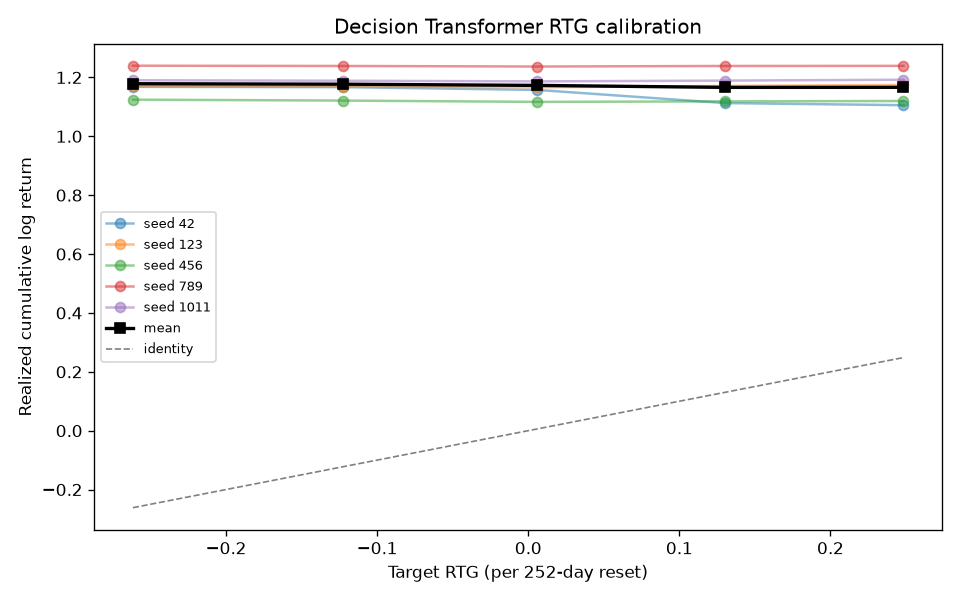
\includegraphics[width=0.72\textwidth]{eval/rtg_calibration.png}
\caption{Return-to-Go calibration for the Decision Transformer. Each coloured line is one seed;
the heavy black line is the seed mean; the dashed grey line is the identity a perfectly
calibrated model would follow (realised return $=$ requested return). The realised curves are
flat: over the entire range of targets the model produces the same allocation policy, and the
mean line drifts slightly \emph{downwards} rather than upwards. The large vertical offset
between the flat realised lines and the identity line is a separate, expected artefact---the
target is a one-year budget while the realised value accumulates over six years---but the
absence of any positive slope is the finding.}
\label{fig:rtgcal}
\end{figure}

\subsubsection{Ablation 3: context length $K$}
\label{sec:ablation-k}

\begin{table}[h]
\centering
\caption{Context-length ablation. The Decision Transformer is retrained from scratch at each
$K$ with every other hyperparameter and the seed (42) held fixed; $K=30$ reuses the main
\texttt{dt\_seed42} checkpoint, whose configuration is identical. Losses are the final training
and best validation action MSE; the remaining columns are the 2020--2025 backtest.}
\label{tab:ablation-k}
\small
\begin{tabular}{rrrrrrrr}
\toprule
$K$ & Tokens $3K$ & Train MSE & Val.\ MSE & Sharpe & CAGR & Max DD & Turnover \\
 & & ($\times 10^{-3}$) & ($\times 10^{-3}$) & & & & \\
\midrule
$10$ & $30$  & $3.202$ & $3.298$ & $\mathbf{0.949}$ & $0.218$ & $-0.288$ & $0.043$ \\
$20$ & $60$  & $3.224$ & $3.303$ & $0.941$ & $0.216$ & $-0.289$ & $0.042$ \\
$30$ & $90$  & $3.242$ & $3.309$ & $0.747$ & $0.203$ & $-0.374$ & $0.136$ \\
$50$ & $150$ & $3.225$ & $3.301$ & $0.667$ & $0.178$ & $-0.378$ & $0.146$ \\
\bottomrule
\end{tabular}
\end{table}

\begin{figure}[t]
\centering
\includegraphics[width=\textwidth]{paper/context_length.png}
\caption{Context-length ablation. \textbf{Left:} final training and best validation action MSE
against $K$. Over a five-fold range of context the loss moves by less than $1\%$
($3.298$--$3.309 \times 10^{-3}$ on validation) and does not decrease with $K$---extra history
buys the model no additional ability to reproduce the behaviour policies. \textbf{Right:} test
Sharpe at each $K$ (seed 42, solid line) against the five individual seeds trained at $K=30$
(light dots, dotted line at their mean $0.966$) and the equal-weight baseline (dashed green).
The seed-42 curve falls steeply with $K$, but the $K=30$ seed cloud spans $0.75$--$1.09$, which
is wider than the $K{=}10$-to-$K{=}20$ gap---so the drop must be read with the caveat in the
text. What the panel does show unambiguously is that no context length, and no seed at any
context length, reaches the baseline.}
\label{fig:ctxlen}
\end{figure}

Table~\ref{tab:ablation-k} and Figure~\ref{fig:ctxlen} vary the one architectural
hyperparameter that is specific to the sequence-modelling framing. Two readings are warranted,
and they differ in how confident we can be.

The \textbf{unambiguous} result is that the imitation loss is flat in $K$. Going from 30 tokens
to 150 changes the best validation MSE by $0.011 \times 10^{-3}$, a relative change of $0.3\%$,
and the ordering is not even monotone. Whatever the transformer is using to predict the next
allocation, it is essentially contained in the most recent ten days; the additional forty days
of context available at $K=50$ are not informative. That is consistent with the state vector
already carrying a 20-day lookback internally (Section~\ref{sec:data}), so a longer token
context largely duplicates information the state encoding provides.

The \textbf{suggestive but confounded} result is the Sharpe column, which falls monotonically
from $0.949$ at $K=10$ to $0.667$ at $K=50$, tracking a jump in mean daily turnover from
$4.3\%$ to $14.6\%$. Taken at face value this would say that longer contexts make the policy
churn. We do not claim that, because the sweep uses one seed per $K$ and the five seeds trained
at $K=30$ are themselves bimodal in exactly this way: seed 42 turns over $13.6\%$ per day and
scores $0.747$, while seeds 123, 456, 789 and 1011 all turn over $4.2$--$4.4\%$ and score
$0.95$--$1.09$. The split is caused by the seed rather than by the model: at seed 42 the RTG-free
control lands in the same high-turnover mode ($12.3\%$, Sharpe $0.81$), and at every other seed
both models land in the low one. The high-turnover mode is therefore a seed-dependent failure
mode that exists at fixed $K$, and with one run per setting we cannot separate it from a genuine effect of $K$. The
honest summary is that the $K=10$ and $K=20$ runs landed in the well-behaved mode and the $K=30$
and $K=50$ runs did not. It is also the one place in this study where a larger compute budget
would clearly have changed what we could conclude: five seeds per $K$ would settle it, and at
roughly 45 minutes per $K=50$ run on a GTX~1070 that was out of reach here.

Two things survive both readings. No context length produced a Sharpe above the $K=30$ five-seed
mean of $0.966$, and none came close to the $1.118$ baseline, so the default $K=30$ is not
leaving performance on the table. And the bimodality itself is worth recording: DT training on
this buffer converges to two distinct policies with indistinguishable imitation loss
($3.3\times 10^{-3}$ in both modes) but a threefold difference in turnover and a $0.3$ difference
in Sharpe. A validation loss computed on held-out \emph{transitions} cannot tell these apart,
which is a concrete argument for selecting offline-RL checkpoints on a backtest statistic rather
than on the training objective.


\subsubsection{Ablation 4: transaction cost sensitivity}
\label{sec:ablation-cost}

\begin{table}[h]
\centering
\caption{Transaction-cost ablation on the test window. Each column re-runs the full backtest
with a different proportional cost $\mu$; DT and BC rows average all five seeds. The
$\Delta$Sharpe column is the Sharpe lost per 25\,bp of additional cost, which tracks the
strategy's mean daily turnover almost exactly.}
\label{tab:cost}
\small
\begin{tabular}{lrrrrrr}
\toprule
& \multicolumn{4}{c}{Sharpe at cost $\mu$} & & \\
\cmidrule(lr){2-5}
Strategy & $0$\,bp & $5$\,bp & $10$\,bp & $25$\,bp & $\Delta$Sharpe / 25\,bp & Turnover \\
\midrule
Buy-and-hold / $1/N$ & $1.118$ & $1.118$ & $1.118$ & $1.118$ & $0.000$ & $\sim 0$ \\
Minimum-variance     & $1.116$ & $1.116$ & $1.116$ & $1.115$ & $-0.001$ & $0.0002$ \\
Mean-variance        & $1.125$ & $1.121$ & $1.116$ & $1.101$ & $-0.024$ & $0.007$ \\
Momentum             & $\mathbf{1.141}$ & $1.057$ & $0.973$ & $0.720$ & $-0.421$ & $0.151$ \\
Transformer BC       & $1.054$ & $1.015$ & $0.976$ & $0.860$ & $-0.194$ & $0.059$ \\
Decision Transformer & $1.047$ & $1.006$ & $0.966$ & $0.845$ & $-0.202$ & $0.061$ \\
\bottomrule
\end{tabular}
\end{table}

\begin{figure}[t]
\centering
\includegraphics[width=\textwidth]{paper/cost_sensitivity.png}
\caption{Sharpe (left) and CAGR (right) against the proportional transaction cost; DT and BC
are means over five seeds. Slopes are proportional to turnover, so the two flat lines are the
near-zero-turnover strategies and the steepest is momentum ($15.1\%$ daily turnover), with DT
($6.1\%$) and BC ($5.9\%$) intermediate. Two crossings matter. In the left panel momentum
starts \emph{above} equal weight at zero cost and falls below it at roughly $1.4$\,bp, so its
entire risk-adjusted edge is a frictionless artefact; in the right panel its raw CAGR advantage
survives until about $17$\,bp. Most importantly, the DT and BC lines never reach the
buy-and-hold line even at the left edge of the plot, where trading is free---about half of their
deficit is not a transaction-cost problem at all.}
\label{fig:cost}
\end{figure}

Table~\ref{tab:cost} and Figure~\ref{fig:cost} separate two explanations that are easy to
conflate. Costs clearly matter, and they matter in direct proportion to turnover: the Sharpe
lost per 25\,bp is $-0.421$ for momentum ($15.1\%$ daily turnover), $-0.202$ and $-0.194$ for DT
and BC ($6.1\%$ and $5.9\%$), $-0.024$ for mean-variance ($0.7\%$) and exactly zero for equal
weight. Momentum is the clearest casualty. At zero cost it is the best strategy anywhere in this
study---Sharpe $1.141$ against equal weight's $1.118$---and that edge is gone by roughly
$1.4$\,bp; only its raw CAGR advantage survives, and only to about $17$\,bp.

But costs do \emph{not} explain the learned models' failure; they explain about half of it. At
$\mu = 0$, where trading is free, DT averages $1.047 \pm 0.096$ and BC $1.054 \pm 0.079$ against
equal weight's $1.118$. Decomposing DT's total deficit of $0.152$ Sharpe at the default
$10$\,bp: $0.072$ of it is holding a worse portfolio than $\mathbf{1}/N$ even when rebalancing
is free, and the remaining $0.081$ is the cost of the churn required to hold it. That is a
useful bound on the obvious fix---a turnover-penalised or trade-throttled DT could recover a
little over half the gap and would still sit behind a policy that does nothing at all.

\subsubsection{Ablation 5: a different asset universe}
\label{sec:universeb}

\begin{table}[h]
\centering
\caption{Universe~B robustness check: Universe~A plus Bitcoin and aluminium ($N=16$), which
forces the data to start on 2014-09-17 and shortens training to two years before the validation
split. The entire pipeline---prepare, trajectories, a fresh $5 \times 8$ training sweep, and
evaluation---was re-run into scoped artefact directories. Test window and cost are unchanged.}
\label{tab:universeb}
\small
\begin{tabular}{lrrrr}
\toprule
Strategy & CAGR & \textbf{Sharpe} & Max DD & Turnover \\
\midrule
Mean-variance        & $0.267$ & $\mathbf{1.202}$ & $-0.265$ & $0.009$ \\
Buy-and-hold / $1/N$ & $0.257$ & $1.202$ & $-0.254$ & ${\sim}0$ \\
PPO$^\dagger$        & $0.257 \pm 0.000$ & $1.202 \pm 0.000$ & $-0.254$ & ${\sim}0$ \\
Minimum-variance     & $0.254$ & $1.200$ & $-0.251$ & $0.0002$ \\
Momentum             & $0.308$ & $1.109$ & $-0.374$ & $0.151$ \\
\textbf{Decision Transformer} & $0.232 \pm 0.016$ & $1.091 \pm 0.117$ & $-0.262 \pm 0.015$ & $0.046$ \\
Transformer BC       & $0.230 \pm 0.019$ & $1.083 \pm 0.127$ & $-0.260 \pm 0.014$ & $0.047$ \\
SAC                  & $0.222 \pm 0.014$ & $1.040 \pm 0.195$ & $-0.293 \pm 0.060$ & $0.064$ \\
CQL                  & $\mathbf{0.652 \pm 0.076}$ & $0.950 \pm 0.079$ & $-0.648 \pm 0.022$ & $0.068$ \\
IQL                  & $0.231 \pm 0.060$ & $0.838 \pm 0.339$ & $-0.393 \pm 0.103$ & $0.121$ \\
TD3+BC               & $0.249 \pm 0.042$ & $0.642 \pm 0.128$ & $-0.460 \pm 0.076$ & $0.143$ \\
A2C                  & $0.189 \pm 0.149$ & $0.340 \pm 0.249$ & $-0.661 \pm 0.125$ & $1.035$ \\
\bottomrule
\end{tabular}
\end{table}

Table~\ref{tab:universeb} repeats the entire study on a universe that adds two assets with very
different dynamics---Bitcoin, which is roughly four times as volatile as the equity sleeve, and
aluminium---and which, because Bitcoin only starts in late 2014, leaves a much shorter training
history. Every qualitative conclusion survives: equal weight is again at the top, no learned
model beats it, CQL again buys a spectacular CAGR ($65.2\%$, driven by an $80.2\%$ average weight in Nvidia plus $13.2\%$
in Bitcoin)
with a catastrophic $-64.8\%$ drawdown and a mediocre Sharpe, PPO again collapses to $1/N$, and
A2C is again unusable. Two differences are worth noting. First, DT now edges \emph{ahead} of BC
($1.091$ vs.\ $1.083$), reversing the Universe~A ordering---but the gap is $0.008$ against seed
standard deviations of $0.12$, so the honest reading is that the two are indistinguishable in
both universes rather than that conditioning helps here. Second, the high-turnover failure mode does not
occur at all in Universe~B: all five DT seeds turn over $4.6\%$ per day, with no outlier. The
$6.1\%$ Universe~A mean in Table~\ref{tab:learned} is entirely the seed-42 outlier, so the
apparent improvement is the \emph{absence} of a bad seed rather than a genuinely more
conservative clone---a shorter, more homogeneous training period seems to make the bad mode
unreachable. The Universe~B
RTG sweep is likewise flat, moving Sharpe from $1.084$ at the 10th percentile to $1.091$ at the
90th---a $+0.007$ slope, nominally in the right direction and numerically irrelevant.

\subsection{Correctness issues that had to be fixed first}
\label{sec:bugs}

Several defects in an early version of the RL baselines made their losses meaningless, and we
record them because they are easy to reproduce and hard to notice. The Bellman target used
$s' = s$, so the critics solved $Q(s) = r + \gamma Q(s)$ and diverged; TD3+BC's target critic
was deep-copied once and never updated; IQL's value function was fitted against the \emph{live}
critic instead of a frozen target and chased itself to a loss of $10^4$; CQL's conservative
penalty took a log-sum-exp over the \emph{batch} rather than over sampled actions, which makes
the penalty approximately $2\log(\text{batch size})$ and independent of the policy; and RL
checkpoints stored the algorithm's name string rather than its weights, so ``loading'' a
checkpoint silently produced a randomly initialised agent. Separately, the transformer's
right-aligned padding mask could mask every key in a query row, producing a softmax over an
empty set and NaN gradients. All are now fixed---real next states from the episode index with
terminal transitions cutting the bootstrap, Polyak targets at $\tau = 0.005$, a frozen target
for IQL's value regression, CQL(H) over ten sampled actions, full module state dicts in
checkpoints, and a guarantee that the attention diagonal is always attendable---and each is
covered by a regression test.

\section{Conclusion}

We asked whether return-conditioned sequence modelling improves offline portfolio allocation,
and built the controls needed to answer it: a Decision Transformer and an architecturally
identical RTG-free control, six value-based and policy-gradient RL baselines, six classical
allocators, five seeds each, a 2{,}580-dimensional state engineered from a public 30-year
daily-close dataset, a 3{,}600-episode offline buffer synthesised from 18 behaviour policies, a
cost-aware log-growth reward, a six-year held-out window, walk-forward folds, block-bootstrap
and Ledoit--Wolf significance tests, and five ablations. The answer on this task is no. No
learned allocator beat cost-aware equal weight (Sharpe $1.118$); the Decision Transformer
reached $0.966 \pm 0.133$ while its RTG-free twin reached $0.976 \pm 0.106$; sweeping the
conditioning target across the full range of training returns moved realised Sharpe by $0.040$
in the wrong direction; a five-fold change in context length moved the imitation loss by
$0.3\%$ and closed none of the gap; removing transaction costs entirely closed only about half
of it;
and a second universe containing Bitcoin reproduced every one of these findings. The most
useful thing we can report is the diagnosis rather than the verdict. An MSE-to-behaviour
objective gives the model no incentive to respond to the Return-to-Go token, and in an
environment whose price process is exogenous there may be no action-conditional route to the
requested return in the first place. Looking at the weights rather than the metrics sharpens
that further: on four of five seeds the trained Decision Transformer's average allocation is
equal weight to within noise, so it has not so much failed to find a good policy as
rediscovered the baseline and then paid transaction costs to maintain it.

\paragraph{Limitations.}
The dataset is close-only, so no volume or microstructure features are possible, and it is a
single (if long) historical path. The environment measures turnover against the previous
\emph{target} weights rather than against mark-to-market drifted holdings, which makes
buy-and-hold and daily-rebalanced equal weight numerically identical and mildly flatters the
baseline; a drifted buy-and-hold was not simulated. The compute budget (one GTX~1070) capped
training at roughly three passes over the buffer rather than full convergence on a large
sweep, and confined hyperparameter exploration to the context-length and cost dimensions.
The context-length sweep in particular runs one seed per $K$, which---given the bimodal turnover
behaviour documented in Section~\ref{sec:ablation-k}---is not enough to attribute its Sharpe
trend to $K$ rather than to seed variation.
PPO, SAC and A2C perform single-step updates over the offline buffer rather than interacting
with a live environment, so they are reference points rather than a fair online comparison.
The deflated Sharpe ratio was computed with a per-seed rather than per-algorithm trial count,
which makes it vacuously zero for every strategy including the baseline. And the universes,
while diversified, contain 14--16 assets; results on a several-hundred-asset cross-section may
differ.

\paragraph{Future work.}
The diagnosis points directly at the remedies. An objective that explicitly penalises
insensitivity to the Return-to-Go token---for example, an auxiliary loss that requires the
predicted allocation to change when $\hat{R}$ is perturbed, or advantage-weighted rather than
plain imitation---would test whether conditioning can be made to work rather than assuming it.
Feeding realised return directly into the reward through a Sharpe-like differentiable utility
\cite{moody2001learning,kisiel2022portfolio} instead of cloning behaviour actions is
the natural alternative.
Turnover-penalised or trade-throttled variants would recover the roughly $0.08$ Sharpe the
transformers lose to costs, and selecting checkpoints on a validation \emph{backtest}
statistic rather than on action MSE would avoid the high-turnover mode that held-out imitation
loss cannot see. Beyond the model, the most valuable extensions are a
mark-to-market turnover model, a larger asset cross-section, richer state features if an
OHLCV dataset is substituted, an algorithm-level deflated Sharpe, and---given how strongly the
2022--23 fold separated momentum from equal weight---an explicit regime-conditional evaluation.

\bibliography{myreferences}
\bibliographystyle{unsrt}

\end{document}
